\subsection{关于紧支集测度的积分}

设 \(\mu\) 是 X 上的一个测度，其支集 \(S = \operatorname{Supp}(\mu)\) 是紧的；开集 \(X - S\) 是可忽略的（§2, No.~2, 命题 5）。对每个函数 \(\mathbf{f}\)（取值于向量空间 \(\mathbf{F}\) 或 \(\overline{\mathbf{R}}\) 中），函数 \(\mathbf{f}\) 与 \(\mathbf{f}\varphi_{\mathrm{S}}\) 因而是等价的（§2, No.~4）；为使 \(\mathbf{f}\) 为 \(\mu\)-可积的（当 \(\mathbf{F}\) 是 Banach 空间时），其充要条件是 \(\mathbf{f}\varphi_{\mathrm{S}}\) 可积，此时有（No.~1）

\[
\int \mathbf {f} d \mu = \int \mathbf {f} \varphi_ {\mathrm{S}} d \mu .\tag{21}
\]

此外，若 \(\mathbf{f}\) 在 \(S\) 上有界，则由 (20) 得出

\[
\left| \int \mathbf {f} d \mu \right| \leqslant \| \mu \| \cdot \sup _ {x \in S} | \mathbf {f} (x) |.\tag{22}
\]

特别地，若 \(\mathbf{f}\) 在 \(X\) 上连续，则 \(\mathbf{f}\) 是 \(\mu\)-可积的，因为 \(\mathbf{f}h \in \mathcal{K}(X;F)\)（其中 \(h \in \mathcal{K}(X;R)\) 是在 \(S\) 上等于 1 的任一函数）（Ch. III, §1, No.~2, 引理 1）。更确切地说：

命题 14. --- 设 X 是一个局部紧空间，F 是一个不退化为 0 的 Banach 空间；给 X 到 F 中的全体连续映射所成的空间 \(\mathcal{C}(\mathrm{X};\mathrm{F})\) 赋以紧收敛拓扑。为使 X 上的测度 \(\mu\) 满足：线性映射 \(\mathbf{f} \mapsto \int \mathbf{f} d\mu\)（\(\mathcal{K}(\mathrm{X};\mathrm{F})\) 到 F 中的）可延拓为 \(\mathcal{C}(\mathrm{X};\mathrm{F})\) 到 F 中的连续线性映射，其充要条件是 \(\operatorname{Supp}(\mu)\) 为紧的；这样的延拓是唯一的，且与 No.~1 中定义的积分一致。

我们刚刚看到，若 \(\mu\) 具有紧支集，则积分 \(\int \mathbf{f}d\mu\) 对每个函数 \(\mathbf{f}\in \mathcal{C}(\mathrm{X};\mathrm{F})\) 都有定义，且映射 \(\mathbf{f}\mapsto \int \mathbf{f}d\mu\)（\(\mathcal{C}(\mathrm{X};\mathrm{F})\) 到 \(\mathrm{F}\) 中的）关于紧收敛拓扑是连续的。反之，假设 \(\mathbf{f}\mapsto \int \mathbf{f}d\mu\) 在 \(\mathcal{K}(\mathrm{X};\mathrm{F})\) 中关于紧收敛拓扑是连续的。那么，存在一个紧集 \(K\subset X\) 和一个数 \(a > 0\)，使得 \(|\mu (\mathbf{f})|\leqslant a\cdot \sup_{x\in K}|\mathbf{f}(x)|\) 对每个函数 \(\mathbf{f}\in \mathcal{K}(\mathrm{X};\mathrm{F})\) 成立；特别地，若 \(\mathbf{g}\in \mathcal{K}(\mathrm{X};\mathrm{F})\) 的支集与 \(K\) 不相交，则 \(\mu (\mathbf{g}) = 0\)。取 \(\mathbf{g} = h\mathbf{a}\)，其中 \(\mathbf{a}\neq 0\) 是 \(\mathrm{F}\) 中的一个向量，而 \(h\in \mathcal{K}(\mathrm{X};\mathbf{C})\)，我们看出，\(\mu (h) = 0\) 对每个函数 \(h\in \mathcal{K}(\mathrm{X};\mathbf{C})\)（其支集与 \(K\) 不相交者）都成立，这就证明了 \(\operatorname {Supp}(\mu)\subset K\)。最后，延拓的唯一性由以下事实得出：\(\mathcal{K}(\mathrm{X};\mathrm{F})\) 在 \(\mathcal{C}(\mathrm{X};\mathrm{F})\) 中关于紧收敛拓扑稠密（Ch. III, §1, No.~2, 命题 4）。

命题 14 使我们可以把 X 上具有紧支集的测度与它在 \(\mathcal{C}(\mathrm{X};\mathbf{C})\) 上的连续延拓等同起来。于是，X 上具有紧支集的测度所成之集可以与对偶空间 \(\mathcal{C}'(\mathrm{X};\mathbf{C})\)（即 Hausdorff 局部凸空间 \(\mathcal{C}(\mathrm{X};\mathbf{C})\) 的对偶）等同。回忆起 \(\mathcal{C}(\mathrm{X};\mathbf{C})\) 是完备的（GT, X, §1, No.~6, 定理 2 的推论 3），但它未必是桶式的（习题 17）。然而，若 X 在无穷远处可数，因而是递增紧集序列 \(\mathrm{K}_n\)（满足 \(\mathrm{K}_n \subset \overset{\circ}{\mathrm{K}}_{n+1}\)）之并，则 \(\mathcal{C}(\mathrm{X};\mathbf{C})\) 的拓扑可由可数的半范数族 \(p_n(f) = \sup_{x \in \mathrm{K}_n} |f(x)|\) 定义，因此在这一情形 \(\mathcal{C}(\mathrm{X};\mathbf{C})\) 是一个 Fréchet 空间。由此，设 \(\mathfrak{S}\) 是 \(\mathcal{C}(\mathrm{X};\mathbf{C})\) 的由有界集组成的任一覆盖，则空间 \(\mathcal{C}'(\mathrm{X};\mathbf{C})\) 关于 \(\mathfrak{S}\)-拓扑是拟完备的（TVS, III, §4, No.~2, 定理 1 的推论 4）。

我们在 \(\mathcal{C}^{\prime}(\mathrm{X};\mathbf{C})\) 上主要考虑紧收敛拓扑（即在 \(\mathcal{C}(\mathrm{X};\mathbf{C})\) 的紧子集上一致收敛的拓扑）。回忆起 \(\mathcal{C}(\mathrm{X};\mathbf{C})\) 的相对紧子集 H 由下列性质刻画（GT, X, §2, No.~5, 定理 2 的推论 3）：

\(1^{\circ}\) H 等度连续；

\(2^{\circ}\) 对每个 \(x \in \mathrm{X}\)，集 \(\mathrm{H}(x)\)——诸 \(f(x)\)（其中 \(f\) 取遍 \(\mathrm{H}\)）所成之集——在 \(\mathbf{C}\) 中有界。

命题 15. --- 设 X 是一个局部紧空间，且对每个 \(x \in X\)，设 \(\varepsilon_{x}\) 是点 x 处的 Dirac 测度。映射 \(x \mapsto \varepsilon_{x}\)（从 X 到 \(\mathcal{C}'(X; \mathbf{C})\) 中）关于 \(\mathcal{C}'(X; \mathbf{C})\) 上的紧收敛拓扑是连续的。

考虑 \(\varepsilon_{x_0}\) 在 \(\mathcal{C}'(\mathrm{X};\mathbf{C})\) 中关于这拓扑的一个邻域，我们可以假定它是这样定义的：取一个数 \(\delta > 0\)、一个紧子集 \(\mathrm{H}\)（属于 \(\mathcal{C}(\mathrm{X};\mathbf{C})\)），并考虑测度 \(\mu\)（\(\mathrm{X}\) 上具有紧支集者）所成的集，其中 \(|\mu(f) - \varepsilon_{x_0}(f)| \leqslant \delta\) 对每个函数 \(f \in \mathrm{H}\) 成立。由于 \(\mathrm{H}\) 等度连续，存在 \(\mathrm{U}\)（\(x_0\) 在 \(\mathrm{X}\) 中的一个邻域），使得关系 \(f \in \mathrm{H}\) 蕴涵 \(|f(x) - f(x_0)| \leqslant \delta\) 对所有 \(x \in \mathrm{U}\) 成立，它也可写成 \(|\varepsilon_x(f) - \varepsilon_{x_0}(f)| \leqslant \delta\)，这就证明了命题。(*)

命题 16. --- 设 K 是 X 的一个紧子集，L 是 X 上支集含于 K 的测度 \(\mu\) 所成的向量空间。在 L 上，由紧收敛拓扑 \(\mathcal{T}\)（\(\mathcal{C}'(X; \mathbf{C})\) 上的）所诱导的拓扑与严格紧收敛拓扑 \(\mathcal{T}'\)（\(\mathcal{M}(X; \mathbf{C})\) 上的）（Ch. III, §1, No.~10）一致。

显然，在 L 上，由 T 诱导的拓扑细于由 \(T'\) 诱导的拓扑。反之，设 H 是 \(\mathcal{C}(\mathrm{X};\mathbf{C})\) 的一个紧子集，h 是 \(\mathcal{K}(\mathrm{X};\mathbf{C})\) 中在 K 上等于 1 的一个函数。显然，由函数 fh（其中 f 取遍 H）所成的集 \(H'\) 在 \(\mathcal{K}(\mathrm{X};\mathbf{C})\) 中是严格紧的，且对每个测度 \(\mu\in L\)，\(\mu(f)=\mu(fh)\) 对每个函数 \(f\in H\) 成立，由此即得结论。

推论 1. --- 对 X 的每个紧子集 K 与每个数 a \textgreater{} 0，X 上的测度 \(\mu\) 所成的集 B，其中 \(\operatorname{Supp}(\mu) \subset K\) 且 \(\|\mu\| \leqslant a\)，它是 \(\mathcal{C}'(X; \mathbf{C})\) 的一个等度连续子集，并且它关于紧收敛拓扑 T 是紧的。

因为，设 H 是 \(\mathcal{C}(\mathrm{X};\mathbf{C})\) 的一个由在 K 上一致有界的函数组成的子集；存在一个数 c\textgreater0，使得 \(|\mu(f)|\leqslant c\cdot\|\mu\|\leqslant ac\) 对每个函数 \(f\in H\) 与每个测度 \(\mu\in B\) 成立（由 (22)）；因此 \(B\subset acH^{\circ}\) 在对偶空间 \(\mathcal{C}'(\mathrm{X};\mathbf{C})\)（\(\mathcal{C}(\mathrm{X};\mathbf{C})\) 的对偶）中成立，这就证明了 B 的等度连续性；B 关于 T 的紧性由以下事实得出：在 B 上，T 与淡拓扑诱导出同一拓扑（命题 16 与 Ch. III, §1, No.~10, 命题 17），并且 B 是淡紧的（Ch. III, §1, No.~9, 命题 15 的推论 2 与 §2, No.~2, 命题 6）。

推论 2. --- 每个具有紧支集的测度（相应地，每个具有紧支集的正测度）\(\mu\) 都属于 \(\mathcal{C}'(\mathrm{X};\mathbf{C})\) 中（关于紧收敛拓扑 \(\mathcal{T}\)）由测度（相应地

正测度）——其支集有限、含于 \(\operatorname{Supp}(\mu)\) 且其范数等于 \(\| \mu \|\)——所成之集的闭包。

因为，在测度 \(\nu\)（满足 \(\operatorname{Supp}(\nu) \subset \operatorname{Supp}(\mu)\) 且 \(\|\nu\| \leqslant \|\mu\|\)）所成的集 B 上，由淡拓扑诱导的拓扑与由 T 诱导的拓扑相同，因此该推论由 Ch. III, §2, No.~4, 定理 1 的推论 2 与 3 得出。

\subsection{集环与加性集函数}

定义 3. --- 一个非空集 \(\Phi\)（集合 \(A\) 的子集所成之集）称为集环，如果存在一个代数 \(\mathcal{A}\)（ \(\mathbf{R}\) 上的），它由定义在 \(A\) 上的实值函数组成，使得关系 \(M \in \Phi\) 与 \(\varphi_{M} \in \mathcal{A}\) 等价。

例. --- 若 \(\mu\) 是局部紧空间 X 上的一个测度，则可积集的特征函数以实数为系数的线性组合构成一个代数 A，因为对任意两个可积集 M、N，函数 \(\varphi_{M}\varphi_{N} = \varphi_{M\cap N}\) 是可积的（No.~5, 命题 7）；于是由定义 2 与定义 3 得出，X 的可积子集所成之集是一个集环。

命题 17. --- 为使集合 A 的子集所成的非空集 \(\Phi\) 是一个集环，其充要条件是它满足下列条件：

\begin{enumerate}
\def\labelenumi{(\Roman{enumi})}
\setcounter{enumi}{149}
\tightlist
\item
  对属于 \(\Phi\) 的每对集合 M、N，集合 \(M\cup N\) 与 \(M\cap CN\) 属于 \(\Phi\)。¹
\end{enumerate}

这条件是必要的，这由关系式

\[
\varphi_ {\mathrm{M} \cup \mathrm{N}} = \varphi_ {\mathrm{M}} + \varphi_ {\mathrm{N}} - \varphi_ {\mathrm{M}} \varphi_ {\mathrm{N}}, \quad \varphi_ {\mathrm{M} \cap \mathbf {C N}} = \varphi_ {\mathrm{M}} - \varphi_ {\mathrm{M}} \varphi_ {\mathrm{N}}.
\]

为证明它是充分的，我们首先注意到它蕴涵：对 \(\Phi\) 中任意两个集合 M、N，M∩N 属于 \(\Phi\)，因为 \(M\cap N=M\cap\mathbb{C}(M\cap\mathbb{C}N)\)。设 \(\mathcal{E}(\Phi)\) 是 \(\Phi\) 中集合的特征函数以实数为系数的线性组合所成之集。由于 \(\varphi_{M}\varphi_{N}=\varphi_{M\cap N}\)，\(\mathcal{E}(\Phi)\) 是一个代数。问题归结为证明：若 M 是 A 的一个子集，使得 \(\varphi_{M}=\sum_{i}c_{i}\varphi_{M_{i}}\) （其中 \(M_{i}\) 属于 \(\Phi\)），则 \(M\in\Phi\)。这将由下面的引理得出：

引理. --- 设 \(\Phi\) 是 A 的子集所成的一个满足公理 (CL) 的非空集。给定一个有限族 \((\mathrm{M}_i)_{1 \leqslant i \leqslant n}\)（由 \(\Phi\) 中的集合组成），存在一个有限族 \((\mathbf{N}_j)_{1\leqslant j\leqslant m}\)（由 \(\Phi\) 中两两不相交的集合组成），使得每个 \(\mathbf{M}_i\) 都是若干个 \(\mathbf{N}_j\) 的并。

因为，考虑 \(2^{n} - 1\) 个形如 \(\bigcap_{i=1}^{n} \mathrm{P}_{i}\) 的集合，其中 \(\mathrm{P}_{i} = \mathrm{M}_{i}\)（对某些指标 \(i\)），\(\mathrm{P}_{i} = \complement \mathrm{M}_{i}\)（对其余的指标），且至少有一个 \(\mathrm{P}_{i}\) 等于 \(\mathrm{M}_{i}\)。设 \((\mathrm{N}_{j})_{1 \leqslant j \leqslant m}\) 是这些集合按某个次序排成的序列；它们两两不相交且属于 \(\Phi\)；另一方面，每个集合 \(\mathrm{M}_{k}\) 是诸集合 \(\mathrm{N}_{j} = \bigcap_{i=1}^{n} \mathrm{P}_{i}\)（对应于族 \((\mathrm{P}_{i})\)，其中 \(\mathrm{P}_{k} = \mathrm{M}_{k}\)）的并，这就证明了引理。

引理证毕，每个形如 \(\sum_{i=1}^{n} c_i \varphi_{\mathrm{M}_i}\) （其中 \(\mathrm{M}_i \in \Phi\)）的函数都可写成 \(\sum_{j=1}^{m} d_j \varphi_{\mathrm{N}_j}\) 的形式，其中 \(\mathrm{N}_j\) 属于 \(\Phi\) 且两两不相交；若 \(\varphi_{\mathrm{M}} = \sum_{j=1}^{m} d_j \varphi_{\mathrm{N}_j}\)，则必有 \(d_j = 0\) 或 \(d_j = 1\)（对每个指标 \(j\)），从而 \(\mathrm{M}\) 是若干个 \(\mathrm{N}_j\) 的并，因此属于 \(\Phi\)。

A 的子集的每个集环 \(\Phi\) 都含有 A 的空子集 \(\varnothing\)；因为至少存在一个子集 \(M \in \Phi\)，因此 \(M - M = \varnothing\) 属于 \(\Phi\)。还应注意，由单独一个子集 \(\varnothing\) 组成的 A 的子集所成之集是一个集环。

定义 4. --- 给定集合 A 的子集所成的一个集环 \(\Phi\) 与一个 Banach 空间 F，我们把阶梯函数\(^{2}\)（在 \(\Phi\) 的集合上的、取值于 F 的；或称 \(\Phi\)-阶梯函数）理解为每个形如 \(\sum_{i} \mathbf{a}_{i} \varphi_{\mathrm{M}_{i}}\) 的函数，其中 \(\mathbf{a}_{i}\) 属于 F，而 \(\mathrm{M}_{i}\) 属于 \(\Phi\)。

显然，集 \(\mathcal{E}_{\mathrm{F}}(\Phi)\)（取值于 F 的 \(\Phi\)-阶梯函数所成之集）是 R 或 C 上的一个向量空间。我们刚才在命题 17 中看到，集 \(\mathcal{E}(\Phi)\)（实值 \(\Phi\)-阶梯函数所成之集）是 R 上的一个代数；它也是 \(R^{A}\) 的由 \(\Phi\) 中集合的特征函数生成的线性子空间。

由该引理，\(\mathcal{E}_{\mathrm{F}}(\Phi)\) 中的每个函数都可写成 \(f = \sum_{j} c_{j} \varphi_{N_{j}}\)，其中 \(N_{j} \in \Phi\) 两两不相交；由此得出 \(|f| = \sum_{j} |c_{j}| \varphi_{N_{j}}\) 属于 \(\mathcal{E}(\Phi)\)。特别地，\(\mathcal{E}(\Phi)\) 是一个 Riesz 空间，因为 \(\mathcal{E}(\Phi)\) 中两个函数的上包络属于 \(\mathcal{E}(\Phi)\)。

注. --- 容易看出，定义 4 等价于下述说法：取值于 F 的 \(\Phi\)-阶梯函数是这样一种函数 f：它只取有限多个值，并且对 F 中每个 \(a \neq 0\)，集合 \(\mathbf{f}^{-1}(a)\) 属于 \(\Phi\)。

定义 5. --- 实值函数 \(\lambda\)（定义在一个集环 \(\Phi\)——集合 \(A\) 的子集所成之集——上）称为加性的，如果对每对不相交的集合 \(M, N\)（它们属于 \(\Phi\)），有 \(\lambda(M \cup N) = \lambda(M) + \lambda(N)\)。

特别地，由这个定义得出 \(\lambda(\varnothing)=0\)。

命题 18. --- 设 \(\lambda\) 是定义在集环 \(\Phi\) 上的一个加性集函数。存在且仅存在一个线性形式（仍记作 \(\lambda\)），它定义在向量空间 \(\mathcal{E}(\Phi)\)（实值 \(\Phi\)-阶梯函数所成的）上，使得 \(\lambda(\varphi_{\mathrm{M}}) = \lambda(\mathrm{M})\) 对每个集合 \(\mathrm{M} \in \Phi\) 成立；此外，若 \(\lambda(\mathrm{M}) \geqslant 0\) 对每个 \(\mathrm{M} \in \Phi\) 成立，则 \(\lambda\) 是 \(\mathcal{E}(\Phi)\) 上的一个正线性形式。

线性形式 \(\lambda\) 的唯一性是明显的，因为 \(\Phi\) 中集合的特征函数生成向量空间 \(\mathcal{E}(\Phi)\)。为证明 \(\lambda\) 的存在性，只需证明关系 \(\sum_{i} c_i \varphi_{\mathrm{M}_i} = 0\) （其中 \(\mathrm{M}_i\) 是属于 \(\Phi\) 的非空集合）蕴涵 \(\sum_{i} c_i \lambda(\mathrm{M}_i) = 0\)。现在，由该引理，存在两两不相交的非空集合的一个有限族 \((\mathrm{N}_j)\)（它们属于 \(\Phi\)），使得对每个指标 \(i\)，有 \(\varphi_{\mathrm{M}_i} = \sum_{j} a_{ij} \varphi_{\mathrm{N}_j}\)，其中 \(a_{ij} = 0\) 或 \(a_{ij} = 1\)。关系 \(\sum_{i} c_i \varphi_{\mathrm{M}_i} = 0\) 可写成 \(\sum_{j} \left( \sum_{i} c_i a_{ij} \right) \varphi_{\mathrm{N}_j} = 0\)，因此它蕴涵 \(\sum_{i} c_i a_{ij} = 0\) 对每个指标 \(j\) 成立。于是由定义 5，我们有

\[
\sum_ {i} c _ {i} \lambda (\mathrm{M} _ {i}) = \sum_ {j} \left(\sum_ {i} c _ {i} a _ {i j}\right) \lambda (\mathrm{N} _ {j}) = 0,
\]

这就证明了 \(\lambda\) 的存在性。最后，假设 \(\lambda(M) \geqslant 0\) 对每个 \(M \in \Phi\) 成立；对每个函数 \(f \in \mathcal{E}(\Phi)\)，可写 \(f = \sum_{i} c_i \varphi_{M_i}\)，其中 \(M_i \in \Phi\) 两两不相交；若 \(f \geqslant 0\)，则由此得出，\(c_i \geqslant 0\) 对每个指标 \(i\)（使得 \(M_i\) 非空者）成立，从而 \(\lambda(f) = \sum_{i} c_i \lambda(M_i) \geqslant 0\)。

\subsection{用阶梯函数逼近连续函数}

命题 19. --- 设 X 是一个局部紧空间，\(\Phi\) 是 X 的子集所成的一个集环，它包含 X 的紧子集全体所成之集。对每个具有紧支集 K 的、X 到 Banach 空间 F 中的连续映射 f（相应地，X 上的每个连续实值函数 \(f \geqslant 0\)），存在函数的一个序列 \((\mathbf{g}_n)\)（属于 \(\mathcal{E}_{\mathrm{F}}(\Phi)\)，其支集含于 K）（相应地，存在函数的一个序列 \((g_n)\)（属于 \(\mathcal{E}(\Phi)\)，使得 \(0 \leqslant g_n \leqslant f\) 对每个 n 成立）），它一致收敛于 f（相应地 \(f\)）。

由于 \(\mathbf{f}\) 在 \(K\) 上一致连续，\(K\) 可被有限个紧集 \(\mathbf{M}_i\) （ \(1 \leqslant i \leqslant m\) ）所覆盖，使得 \(\mathbf{f}\) 在每个 \(\mathbf{M}_i\) 上的振幅 \(\leqslant 1/n\)。由于 \(\mathbf{M}_i\) 与 \(K\) 属于 \(\Phi\)，存在把 \(K\) 分成集合 \(\mathbf{N}_j \in \Phi\) 的一个分割，使得每个集合 \(\mathbf{M}_i \cap K\) 是若干个 \(\mathbf{N}_j\) 的并（No.~9, 引理）。设 \(\mathbf{a}_j\) 是 \(F\) 的一个元素，使得 \(|\mathbf{f}(x) - \mathbf{a}_j| \leqslant 1/n\) 在 \(\mathbf{N}_j\) 上成立。令 \(\mathbf{g}_n = \sum_j \mathbf{a}_j \varphi_{\mathbf{N}_j}\)，我们就有 \(|\mathbf{f} - \mathbf{g}_n| \leqslant 1/n\)，由此得到该命题在这一情形的结论。对连续实值函数 \(f\) 可类似论证，只需取 \(a_j = \inf_{x \in \mathbb{N}_j} f(x)\) 与 \(g_n = \sum_j a_j \varphi_{\mathbf{N}_j}\)。

推论 1. --- 设 \(\mu\) 是 X 上的一个测度；空间 \(\mathcal{E}_{\mathrm{F}}(\Phi)\) 在每个空间 \(\mathcal{L}_{\mathrm{F}}^{p}\) （ \(1 \leqslant p < +\infty\)）中稠密。

因为，由命题 19 以及具有紧支集的函数的一致极限的平均收敛准则（§3, No.~3, 命题 4）得出，\(\mathcal{E}_{\mathrm{F}}(\Phi)\) 关于 \(p\) 阶平均收敛拓扑，在具有紧支集的连续函数所成的空间 \(\mathcal{K}_{\mathrm{F}}\) 的闭包中稠密，由此即得该推论。

推论 2. --- 对 X 的每个闭子集 S，每个函数 \(f \in \mathcal{K}(X, S; \mathbf{C})\) 都是线性组合 \(\sum_{i} \lambda_i \varphi_{K_i}\) 的一致极限，其中 \(\lambda_i\) 属于 \(\mathbf{C}\)，而 \(K_i\) 是 \(S\) 的紧子集。

这种线性组合所成之集 A 是一个 C-代数。设 \(\Phi\) 是 X 的使 \(\varphi_{M} \in A\) 的子集 M 所成之集；这样 \(\Phi\) 就是一个集环，其所有元素都是 S 的子集，它包含 S 的紧子集，并且 \(\mathcal{E}_{\mathbf{C}}(\Phi) \subset \mathcal{A}\)。于是只需对局部紧空间 S 与集环 \(\Phi\) 应用命题 19。

推论 3. --- 若 \(\mu\) 与 \(\nu\) 是 X 上的两个测度，使得 \(\mu(K) = \nu(K)\) 对每个紧子集 \(K\)（\(X\) 的）成立，则 \(\mu = \nu\)。

因为，由推论 2 与测度的定义得出，对 X 的每个紧子集 S，\(\mu\) 与 \(\nu\) 在 \(\mathcal{K}(\mathrm{X},\mathrm{S};\mathbf{C})\) 上取相同的值。

\subsection{定义在集族上的测度的延拓}

设 \(\Phi\) 是局部紧空间 \(X\) 的子集所成的一个非空集。给定一个实值函数 \(M \mapsto \alpha(M)\)，它有定义且 \(\geqslant 0\) 于 \(\Phi\) 上，我们提出寻求这样的条件：在这些条件下，存在一个正测度 \(\mu\)（\(X\) 上的），使得 \(\Phi\) 中的集合都是 \(\mu\)-可积的，并且 \(\mu(M) = \alpha(M)\) 对所有 \(M \in \Phi\) 成立。我们将只考虑集 \(\Phi\) 满足下列条件的情形：

\((\mathrm{PC}_{\mathrm{I}})\) \(\Phi\) 中两个集合的并与交属于 \(\Phi\)。

\((\mathrm{PC}_{\mathrm{II}})\) 对每个由紧集 \(K\) 与开集 \(U\)（\(X\) 中满足 \(K \subset U\) 者）组成的对，存在一个集合 \(M \in \Phi\)，使得 \(K \subset M \subset U\)。

注意，条件 \((\mathrm{PC}_{\mathrm{II}})\) 蕴涵 \(\varnothing\in\Phi\)，这只需取 \(K=U=\varnothing\)。然而，集 \(\Phi\) 未必是一个集环；例如，X 的所有紧子集所成之集满足条件 \((\mathrm{PC}_{\mathrm{I}})\) 与 \((\mathrm{PC}_{\mathrm{II}})\)，但一般说来不是一个集环，因为若 M 与 N 是紧的，则 \(M\cap \complement N\) 一般说来并不如此。

我们还将假设函数 \(\alpha\)（定义在 \(\Phi\) 上）满足下列条件（它们显然是该问题有解的必要条件）：

\((\mathrm{PM}_{\mathrm{I}})\) 关系 \(\mathrm{M}\subset \mathrm{N}\) 蕴涵 \(\alpha (\mathrm{M})\leqslant \alpha (\mathrm{N})\)

\((\mathrm{PM}_{\mathrm{II}})\) 对 \(\Phi\) 中任意的 M 与 N，\(\alpha (\mathrm{M}\cup \mathrm{N})\leqslant \alpha (\mathrm{M}) + \alpha (\mathrm{N})\)

\((\mathrm{PM}_{\mathrm{III}})\) 关系 \(\mathrm{M}\cap \mathrm{N} = \emptyset\) 蕴涵 \(\alpha (\mathrm{M}\cup \mathrm{N}) = \alpha (\mathrm{M}) + \alpha (\mathrm{N})\)

取 \(\mathbf{N} = \varnothing\) 于条件 \((\mathrm{PM}_{\mathrm{III}})\) 中，可推出 \(\alpha(\varnothing) = 0\)；于是条件 \((\mathrm{PM}_{\mathrm{I}})\) 表明，\(\alpha(M) \geqslant 0\) 对每个 \(M \in \Phi\) 成立。

定理 5. --- 设 \(\Phi\) 是局部紧空间 \(X\) 的子集所成的一个集，满足 \((\mathrm{PC}_{\mathrm{I}})\) 与 \((\mathrm{PC}_{\mathrm{II}})\)，并设 \(\alpha\) 是定义在 \(\Phi\) 上的实值函数，满足条件 \((\mathrm{PM}_{\mathrm{I}})\)、\((\mathrm{PM}_{\mathrm{II}})\) 与 \((\mathrm{PM}_{\mathrm{III}})\)。为使存在一个正测度 \(\mu\)（\(X\) 上的），使得 \(\Phi\) 中的集合都是 \(\mu\)-可积的，并且 \(\mu(M) = \alpha(M)\) 对所有 \(M \in \Phi\) 成立，其充要条件是 \(\alpha\) 还满足下列条件：

\((PM_{IV})\) 对每个 \(\varepsilon > 0\) 与每个 \(M \in \Phi\)，存在一个紧集 \(K \subset M\) 与一个开集 \(U \supset M\)，使得对每个 \(N \in \Phi\)（满足关系 \(K \subset N \subset U\) 者），有 \(|\alpha(N) - \alpha(M)| \leqslant \varepsilon\)。

此外，若条件 \((\mathrm{PM}_{\mathrm{IV}})\) 得到满足，则测度 \(\mu\) 是唯一的；对每个紧集 K，\(\mu(\mathrm{K}) = \inf_{\mathrm{M} \in \Phi, \mathrm{M} \supset \mathrm{K}} \alpha(\mathrm{M})\)；对每个开集 U，\(\mu^{*}(\mathrm{U}) =\)

sup \(\alpha (\mathbf{M})\)

\(\mathbf{M}\in \Phi ,\bar{\mathbf{M}}\subset \mathbf{U}\)

注意，条件 \((PM_{IV})\) 等价于下列两个条件的合取：

\((\mathrm{PM}_{\mathrm{IV}}^{\prime})\) 对每个 \(\varepsilon > 0\) 与每个 \(\mathbf{M} \in \Phi\)，存在一个开集 \(\mathbf{U} \supset \mathbf{M}\)，使得对每个 \(\mathbf{N} \in \Phi\)（含于 \(\mathbf{U}\) 者），有 \(\alpha(\mathbf{N}) \leqslant \alpha(\mathbf{M}) + \varepsilon\)。 \((\mathrm{PM}_{\mathrm{IV}}^{\prime \prime})\) 对每个 \(\varepsilon > 0\) 与每个 \(\mathbf{M} \in \Phi\)，存在一个紧集 \(\mathbf{K} \subset \mathbf{M}\)，使得对每个 \(\mathbf{N} \in \Phi\)（包含 \(\mathbf{K}\) 者），有 \(\alpha(\mathbf{N}) \geqslant \alpha(\mathbf{M}) - \varepsilon\)。

因为，显然 \((\mathrm{PM}_{\mathrm{IV}}^{\prime})\) 与 \((\mathrm{PM}_{\mathrm{IV}}^{\prime\prime})\) 蕴涵 \((\mathrm{PM}_{\mathrm{IV}})\)。反之，例如让我们证明 \((\mathrm{PM}_{\mathrm{IV}})\) 蕴涵 \((\mathrm{PM}_{\mathrm{IV}}^{\prime})\)：设 K 是一个紧集，U 是一个开集，使得 \(K \subset M \subset U\)，并且 \(|\alpha(P) - \alpha(M)| \leqslant \varepsilon\) 对每个 \(P \in \Phi\)（满足 \(K \subset P \subset U\) 者）成立。那么，若 \(N \in \Phi\) 且 \(N \subset U\)，则 \(M \cup N\) 属于 \(\Phi\) 且 \(K \subset M \cup N \subset U\)，于是 \(\alpha(M \cup N) \leqslant \alpha(M) + \varepsilon\)，从而更有 \(\alpha(N) \leqslant \alpha(M) + \varepsilon\)。

当集 \(\Phi\)（满足 \((\mathrm{PC}_{1})\) 与 \((\mathrm{PC}_{11})\) 的）由紧集组成时，条件 \((\mathrm{PM}_{\mathrm{IV}}^{\prime \prime})\) 平凡地成立，于是 \((\mathrm{PM}_{\mathrm{IV}})\) 等价于 \((\mathrm{PM}_{\mathrm{IV}}^{\prime})\)。

条件 \((\mathrm{PM}_{\mathrm{IV}})\) 是必要的：这由 No.~6 的定理 4（关于用紧集与开集“逼近”可积集）立即得出。为证明定理的其余断言，我们分几步进行。

\(1^{\circ}\) \(\mathfrak{P}(\mathrm{X})\) 上一个拓扑的定义。

对由 X 的紧集 K 与开集 U 组成的每个对 \((K,U)\)，我们用 \(I(K,U)\) 表示子集 \(M \subset X\)（满足 \(K \subset M \subset U\) 者）所成之集；为使 \(I(K,U)\) 非空，其充要条件是 \(K \subset U\)。若 \((K',U')\) 是由紧集 \(K'\) 与开集 \(U'\) 组成的第二个对，则我们有

\[
\mathrm{I} (\mathrm{K}, \mathrm{U}) \cap \mathrm{I} (\mathrm{K} ^ {\prime}, \mathrm{U} ^ {\prime}) = \mathrm{I} (\mathrm{K} \cup \mathrm{K} ^ {\prime}, \mathrm{U} \cap \mathrm{U} ^ {\prime}).
\]

设 \(\mathcal{T}\) 是 \(\mathfrak{P}(\mathrm{X})\) 上由诸子集 I(K,U)（当 K 取遍 X 的紧子集所成之集而 U 取遍开子集所成之集时）生成的拓扑；由前所述，诸 I(K,U) 构成拓扑 \(\mathcal{T}\) 的一个基（GT, I, §1, No.~3）。

我们注意到，\(\mathcal{T}\) 的定义蕴涵：在 \(\mathfrak{P}(\mathrm{X})\) 中，\(\mathrm{X}\) 的紧子集所成之集是稠密的。条件 \((\mathrm{PC}_{\mathrm{II}})\) 表达的是 \(\Phi\) 在 \(\mathfrak{P}(\mathrm{X})\) 中稠密，而条件 \((\mathrm{PM}_{\mathrm{IV}})\) 表达的是函数 \(\alpha\) 在 \(\Phi\) 上关于由 \(\mathcal{T}\) 诱导的拓扑连续。最后，No.~6 的定理 4 表达的是：函数 \(\mathrm{M} \mapsto \mu(\mathrm{M})\) 在 \(\mu\)-可积集所成的集环上关于由 \(\mathcal{T}\) 诱导的拓扑连续。

\(2^{\circ}\) \(\mu\) 的唯一性。

我们用 \(\overline{\Phi}\) 表示满足下述条件的子集 \(M \subset X\) 所成之集：\(\alpha(N)\) 当 N（关于拓扑 T）趋于 M 而保持在 \(\Phi\) 中时，趋于一个有限极限；于是我们可以把 \(\alpha\) 以唯一的方式延拓为一个连续映射 \(\overline{\alpha}\)（\(\overline{\Phi}\) 到 R 中的）（GT, I, §8, No.~5, 定理 1）。若存在一个满足所要求条件的测度 \(\mu\)，则上面的注记证明，集环 \(\Psi\)（\(\mu\)-可积集所成者）含于 \(\overline{\Phi}\)，并且 \(\mu(M) = \overline{\alpha}(M)\) 对每个 \(M \in \Psi\) 成立；这一关系特别地对 X 的每个紧子集 M 成立，这就证明了 \(\mu\) 的唯一性（No.~10, 命题 19 的推论 3）。

\(3^{\circ}\) \(\alpha\) 到紧集的延拓。

现在我们将在不假设 \(\mu\) 存在的情况下，研究集 \(\overline{\Phi}\) 以及延拓 \(\overline{\alpha}\)（\(\alpha\) 到 \(\overline{\Phi}\) 上的）。我们首先证明每个紧集 \(K\) 都属于 \(\overline{\Phi}\)，并且 \(\overline{\alpha}(K) = \inf_{P \in \Phi, P \supset K} \alpha(P)\)。设 \(a = \inf_{P \in \Phi, P \supset K} \alpha(P)\)；对每个 \(\varepsilon > 0\)，存在一个 \(M \in \Phi\)，使得 \(K \subset M\) 且 \(\alpha(M) \leqslant a + \varepsilon\)。由 \((PM_{IV}')\)，存在一个开集 \(U \supset M\)，使得对每个 \(N \in \Phi\)（含于 \(U\) 者），有 \(\alpha(N) \leqslant \alpha(M) + \varepsilon \leqslant a + 2\varepsilon\)；于是对每个 \(N \in \Phi\)（满足 \(K \subset N \subset U\) 者），有 \(a \leqslant \alpha(N) \leqslant a + 2\varepsilon\)，这按定义表明 \(K \in \overline{\Phi}\) 且 \(\overline{\alpha}(K) = a\)。

这一结果立即表明，若 \(K_{1}\) 与 \(K_{2}\) 是使 \(K_{1} \subset K_{2}\) 的两个紧集，则 \(\overline{\alpha}(K_{1}) \leqslant \overline{\alpha}(K_{2})\)。若 \(K_{1}\) 与 \(K_{2}\) 是任意两个紧集，则有 \(\overline{\alpha}(K_{1} \cup K_{2}) \leqslant \overline{\alpha}(K_{1}) + \overline{\alpha}(K_{2})\)（由 \((\mathrm{PM}_{\mathrm{II}})\)）。此外，我们还将看到，若 \(K_{1}\) 与 \(K_{2}\) 不相交，则 \(\overline{\alpha}(K_{1} \cup K_{2}) = \overline{\alpha}(K_{1}) + \overline{\alpha}(K_{2})\)。因为此时存在两个不相交的开集 \(U_{1}, U_{2}\)，使 \(K_{1} \subset U_{1}, K_{2} \subset U_{2}\)（GT, II, §4, 命题 4）。于是由 \((\mathrm{PC}_{\mathrm{II}})\)，还存在两个集合 \(M_{1} \in \Phi, M_{2} \in \Phi\)，使 \(K_{1} \subset M_{1} \subset U_{1}\) 且 \(K_{2} \subset M_{2} \subset U_{2}\)。现设 P 是 \(\Phi\) 中包含 \(K_{1} \cup K_{2}\) 的任一集合；两个集合 \(P \cap M_{1}\) 与 \(P \cap M_{2}\) 的并属于 \(\Phi\)（由 \((\mathrm{PC}_{\mathrm{I}})\)），且由于这两个集合不相交，应用 \((\mathrm{PM}_{\mathrm{I}})\) 与 \((\mathrm{PM}_{\mathrm{III}})\) 便得

\[
\alpha (\mathrm{P}) \geqslant \alpha (\mathrm{P} \cap \mathrm{M} _ {1}) + \alpha (\mathrm{P} \cap \mathrm{M} _ {2}) \geqslant \overline {{\alpha}} (\mathrm{K} _ {1}) + \overline {{\alpha}} (\mathrm{K} _ {2}),
\]

由此便建立了我们的断言。

\(4^{\circ}\) \(\alpha\) 到开集的延拓。

现在我们将看到，为使一个开集 U 属于 \(\overline{\Phi}\)，其充要条件是：当 K 取遍 U 的紧子集所成之集时，诸数 \(\overline{\alpha}(K)\) 的上确界有限；此外，此时 \(\overline{\alpha}(U)\) 等于这个上确界。

因为，设 U 是属于 \(\bar{\Phi}\) 的一个开集；对每个 \(\varepsilon > 0\)，存在一个紧集 \(K \subset U\)，使得对每个集合 \(M \in \Phi\)（满足 \(K \subset M \subset U\) 者），有 \(|\overline{\alpha}(U) - \alpha(M)| \leqslant \varepsilon\)，从而 \(|\overline{\alpha}(U) - \overline{\alpha}(K)| \leqslant \varepsilon\)；另一方面，若 \(K'\) 是含于 U 的任一紧集，则 \(K \subset K \cup K' \subset U\)，于是 \(|\overline{\alpha}(U) - \overline{\alpha}(K \cup K')| \leqslant \varepsilon\)，从而 \(\overline{\alpha}(U) \geqslant \overline{\alpha}(K \cup K') - \varepsilon \geqslant \overline{\alpha}(K') - \varepsilon\)；因此 \(\overline{\alpha}(U)\) 确实等于当 K 取遍 U 的紧子集所成之集时诸数 \(\overline{\alpha}(K)\) 的上确界。

反之，设 U 是使 \(b = \sup_{K \subset U} \overline{\alpha}(K) < +\infty\) 的一个开集（其中 K 取

遍 U 的紧子集所成之集），我们来证明 \(U \in \overline{\Phi}\)。对每个 \(\varepsilon > 0\)，存在一个紧集 \(K \subset U\)，使 \(b - \varepsilon \leqslant \overline{\alpha}(K) \leqslant b\)；由 \((\mathrm{PM}_{\mathrm{IV}}^{\prime\prime})\)，对每个集合 \(M \in \Phi\)（满足 \(K \subset M \subset U\) 者），存在一个紧集 \(K' \subset M\)，使得

\[
\alpha (\mathrm{M}) \leqslant \overline {{{{\alpha}}}} (\mathrm{K} ^ {\prime}) + \varepsilon \leqslant b + \varepsilon ;
\]

因此 \(b - \varepsilon \leqslant \alpha (\mathrm{M}) \leqslant b + \varepsilon\)，这就证明了 \(\mathrm{U} \in \overline{\Phi}\)。

由开集 \(U \in \overline{\Phi}\) 以及 \(\overline{\alpha}(U)\) 的这一刻画，首先得出：若 \(U_{1}\) 与 \(U_{2}\) 是使 \(U_{1} \subset U_{2}\) 且 \(U_{2} \in \overline{\Phi}\) 的两个开集，则 \(U_{1} \in \overline{\Phi}\) 且 \(\overline{\alpha}(U_{1}) \leqslant \overline{\alpha}(U_{2})\)。另一方面，若 \(U_{1}\) 与 \(U_{2}\) 是属于 \(\overline{\Phi}\) 的两个开集，则 \(U_{1} \cup U_{2}\) 亦然，且 \(\overline{\alpha}(U_{1} \cup U_{2}) \leqslant \overline{\alpha}(U_{1}) + \overline{\alpha}(U_{2})\)。因为，设 K 是含于 \(U_{1} \cup U_{2}\) 的任一紧集；对每个点 \(x \in K\)，存在 x 的一个含于 \(U_{1}\) 或 \(U_{2}\) 之一的紧邻域；因此可以用有限个这样的邻域覆盖 K；若 \(K_{1}\) （相应地 \(K_{2}\)）是含于 \(U_{1}\) （相应地 \(U_{2}\)）的那些邻域的并，则 \(K \subset K_{1} \cup K_{2}\)，于是

\[
\overline {{{{\alpha}}}} (\mathrm{K}) \leqslant \overline {{{{\alpha}}}} (\mathrm{K} _ {1} \cup \mathrm{K} _ {2}) \leqslant \overline {{{{\alpha}}}} (\mathrm{K} _ {1}) + \overline {{{{\alpha}}}} (\mathrm{K} _ {2}) \leqslant \overline {{{{\alpha}}}} (\mathrm{U} _ {1}) + \overline {{{{\alpha}}}} (\mathrm{U} _ {2}),
\]

由此便建立了所述的性质。

\(5^{\circ}\) \(\overline{\Phi}\) 与 \(\overline{\alpha}\) 的性质。

\(\overline{\Phi}\) 与 \(\overline{\alpha}\) 的定义现在可以改述如下（考虑到 \((\mathrm{PC}_{\mathrm{II}})\)）：为使 \(M \in \overline{\Phi}\)，其充要条件是，对每个 \(\varepsilon > 0\)，存在一个紧集 K 与一个开集 \(U \in \overline{\Phi}\)，使得 \(K \subset M \subset U\) 且 \(\overline{\alpha}(U) - \overline{\alpha}(K) \leqslant \varepsilon\)；此外，\(\overline{\alpha}(M)\) 是诸 \(\overline{\alpha}(U)\)（对应于包含 M 的开集 \(U \in \overline{\Phi}\)）的下确界，以及诸 \(\overline{\alpha}(K)\)（对应于紧集 \(K \subset M\)）的上确界。

由此我们首先推出：若 \(\mathrm{M}_1\)、\(\mathrm{M}_2\) 与 \(\mathrm{M}_1 \cup \mathrm{M}_2\) 属于 \(\overline{\Phi}\)，则 \(\overline{\alpha}(\mathrm{M}_1 \cup \mathrm{M}_2) \leqslant \overline{\alpha}(\mathrm{M}_1) + \overline{\alpha}(\mathrm{M}_2)\)。的确，若 \(\mathrm{U}_1\) 与 \(\mathrm{U}_2\) 是 \(\overline{\Phi}\) 的两个开集，分别包含 \(\mathbf{M}_1\) 与 \(\mathbf{M}_2\)，并且使 \(\overline{\alpha} (\mathrm{U}_1)\leqslant \overline{\alpha} (\mathrm{M}_1) + \varepsilon\) 与 \(\overline{\alpha} (\mathrm{U}_2)\leqslant \overline{\alpha} (\mathrm{M}_2) + \varepsilon\)，则 \(\mathrm{U}_1\cup \mathrm{U}_2\) 属于 \(\overline{\Phi}\)，包含 \(\mathbf{M}_1\cup \mathbf{M}_2\)，从而

\[
\overline {{\alpha}} \left(\mathrm{M} _ {1} \cup \mathrm{M} _ {2}\right) \leqslant \overline {{\alpha}} \left(\mathrm{U} _ {1} \cup \mathrm{U} _ {2}\right) \leqslant \overline {{\alpha}} \left(\mathrm{U} _ {1}\right) + \overline {{\alpha}} \left(\mathrm{U} _ {2}\right) \leqslant \overline {{\alpha}} \left(\mathrm{M} _ {1}\right) + \overline {{\alpha}} \left(\mathrm{M} _ {2}\right) + 2 \varepsilon ,
\]

由此即得我们的断言。

其次，我们来证明：若 \(K\) 是紧集而 \(U\) 是 \(\overline{\Phi}\) 的使 \(K \subset U\) 的开集，则 \(\overline{\alpha}(U - K) = \overline{\alpha}(U) - \overline{\alpha}(K)\)。由前所述，我们有 \(\overline{\alpha}(U) \leqslant \overline{\alpha}(K) + \overline{\alpha}(U - K)\)。另一方面，对每个紧集 \(K' \subset U - K\)，

\[
\overline {{{{\alpha}}}} (\mathrm{K} \cup \mathrm{K} ^ {\prime}) = \overline {{{{\alpha}}}} (\mathrm{K}) + \overline {{{{\alpha}}}} (\mathrm{K} ^ {\prime}) \leqslant \overline {{{{\alpha}}}} (\mathrm{U});
\]

由于 U - K 是开集且属于 \(\overline{\Phi}\)，\(\overline{\alpha}(U - K)\) 是诸 \(\overline{\alpha}(K')\) 的上确界，这表明 \(\overline{\alpha}(K) + \overline{\alpha}(U - K) \leqslant \overline{\alpha}(U)\)。

因此，\(\overline{\Phi}\) 的定义现在可以表述如下：为使 \(M \in \overline{\Phi}\)，其充要条件是，对每个 \(\varepsilon > 0\)，存在一个紧集 K 与一个开集 \(U \in \overline{\Phi}\)，使得 \(K \subset M \subset U\) 且 \(\overline{\alpha}(U - K) \leqslant \varepsilon\)。

现在我们能够证明 \(\overline{\Phi}\) 是一个集环，而 \(\overline{\alpha}\) 是 \(\overline{\Phi}\) 上的一个加性集函数。我们首先证明：若 M 与 N 属于 \(\overline{\Phi}\)，则 M \(\cap\) CN 与 M \(\cup\) N 亦然。按假设，对每个 \(\varepsilon > 0\)，存在两个紧集 K,K' 与 \(\overline{\Phi}\) 的两个开集 U,U'，使得

\[
\mathrm{K} \subset \mathrm{M} \subset \mathrm{U}, \quad \mathrm{K} ^ {\prime} \subset \mathrm{N} \subset \mathrm{U} ^ {\prime}, \quad \overline {{\alpha}} (\mathrm{U} - \mathrm{K}) \leqslant \varepsilon , \quad \overline {{\alpha}} (\mathrm{U} ^ {\prime} - \mathrm{K} ^ {\prime}) \leqslant \varepsilon .
\]

集合 \(K'' = K \cap C U'\) 是紧的，集合 \(U'' = U \cap C K'\) 是开集且属于 \(\overline{\Phi}\)，并且 \(K'' \subset M \cap C N \subset U''\)；另一方面，\(U'' - K''\) 含于 \(U \cap C K\) 与 \(U' \cap C K'\) 的并，于是 \(\overline{\alpha}(U'' - K'') \leqslant 2\varepsilon\)，这就证明了 \(M \cap C N \in \overline{\Phi}\)。类似地，\(U_1 = U \cup U'\) 是开集且属于 \(\overline{\Phi}\)，\(K_1 = K \cup K'\) 是紧的，且 \(K_1 \subset M \cup N \subset U_1\)；另一方面，\(U_1 - K_1\) 含于 U - K 与 \(U' - K'\) 的并，于是同样有 \(\overline{\alpha}(U_1 - K_1) \leqslant 2\varepsilon\)，从而 \(M \cup N\) 属于 \(\overline{\Phi}\)。最后，若 M 与 N 不相交，则

\[
\overline {{{{\alpha}}}} \left(\mathrm{K} _ {1}\right) = \overline {{{{\alpha}}}} (\mathrm{K}) + \overline {{{{\alpha}}}} \left(\mathrm{K} ^ {\prime}\right) \geqslant \overline {{{{\alpha}}}} (\mathrm{M}) + \overline {{{{\alpha}}}} (\mathrm{N}) - 2 \varepsilon ,
\]

因而 \(\overline{\alpha} (\mathbf{M}\cup \mathbf{N})\geqslant \overline{\alpha} (\mathbf{M}) + \overline{\alpha} (\mathbf{N}) - 2\varepsilon\)；由于 \(\varepsilon\) 是任意的，我们有 \(\overline{\alpha} (\mathbf{M}\cup \mathbf{N}) = \overline{\alpha} (\mathbf{M}) + \overline{\alpha} (\mathbf{N})\)

\(6^{\circ}\) 测度 \(\mu\) 的存在性。

由 No.~9 的命题 18，存在且仅存在一个正线性形式 \(\beta\)，它定义在向量空间 \(\mathcal{E}(\overline{\Phi})\)（\(\overline{\Phi}\)-阶梯函数所成的）上，使得 \(\beta(\varphi_{\mathrm{M}}) = \overline{\alpha}(\mathrm{M})\) 对所有 \(\mathrm{M} \in \overline{\Phi}\) 成立。对每个紧子集 \(\mathrm{K}\)（\(\mathrm{X}\) 中的），我们用 \(\mathcal{G}(\mathrm{K})\) 表示 \(\mathcal{E}(\overline{\Phi})\) 中支集含于 \(\mathrm{K}\) 的函数的一致极限所成的空间。由于 \(\beta\) 是正的，\(|\beta(f)| \leqslant \overline{\alpha}(\mathrm{K}) \cdot \|f\|\) 对每个函数 \(f \in \mathcal{E}(\overline{\Phi})\)（支集含于 \(\mathrm{K}\) 者）成立；\(\beta\) 在这些函数所成的空间上的限制是关于一致收敛拓扑的一个连续线性形式；因此它可以延拓为一个正连续线性形式 \(\overline{\beta}_{K}\)（\(\mathcal{G}(K)\) 上的）。此外，若 K 与 \(K_{1}\) 是使 \(K \subset K_{1}\) 的两个紧集，则 \(\overline{\beta}_{K_{1}}\) 在 \(\mathcal{G}(K)\) 上的限制与 \(\overline{\beta}_{K}\) 相同，因此存在一个正线性形式 \(\overline{\beta}\)（在诸 \(\mathcal{G}(K)\) 的并 G 上），它延拓每一个形式 \(\overline{\beta}_{K}\)。

现在，由于每个紧集都属于 \(\overline{\Phi}\)，具有紧支集的连续实值函数所成的空间 \(\mathcal{K}\) 是 \(\mathcal{G}\) 的一个子空间（No.~10, 命题 19）；因此，\(\mathcal{K}\) 上的正线性形式 \(\overline{\beta}\) 的限制是一个正测度 \(\mu\)。我们来证明，对每个紧集 \(K\)，有 \(\mu(K) = \overline{\alpha}(K)\)。对每个 \(\varepsilon > 0\)，存在一个开集 \(U \in \overline{\Phi}\)，使得 \(K \subset U\)，\(\mu(U) \leqslant \mu(K) + \varepsilon\) 且 \(\overline{\alpha}(U) \leqslant \overline{\alpha}(K) + \varepsilon\)。设 \(f\) 是 \(X\) 到 {[}0,1{]} 中的一个连续映射，其支集含于 \(U\)，且 \(f(x) = 1\) 在 \(K\) 上成立（Ch. III, §1, No.~2, 引理 1）。那么 \(\mu(K) \leqslant \mu(f) \leqslant \mu(U) \leqslant \mu(K) + \varepsilon\)，而另一方面，

\[
\overline {{\alpha}} (\mathrm{K}) = \beta (\varphi_ {\mathrm{K}}) \leqslant \overline {{\beta}} (f) \leqslant \beta (\varphi_ {\mathrm{U}}) = \overline {{\alpha}} (\mathrm{U}) \leqslant \overline {{\alpha}} (\mathrm{K}) + \varepsilon ;
\]

由于 \(\mu(f) = \overline{\beta}(f)\)，我们看出 \(|\mu(\mathrm{K}) - \overline{\alpha}(\mathrm{K})| \leqslant \varepsilon\)，又因 \(\varepsilon\) 是任意的，故 \(\mu(\mathrm{K}) = \overline{\alpha}(\mathrm{K})\)。

属于 \(\overline{\Phi}\) 的开集的上述刻画，与 No.~6 的定理 4 的推论 4 相结合，便表明属于 \(\overline{\Phi}\) 的开集恰恰就是 \(\mu\)-可积的开集，并且对这样的集合 U，有 \(\mu(\mathrm{U}) = \overline{\alpha}(\mathrm{U})\)。No.~6 的定理 4 与 \(\overline{\Phi}\) 的集合在 \(5^{\circ}\) 中给出的刻画进而表明，\(\mu\)-可积集就是 \(\overline{\Phi}\) 中的集合，并且对这样的集合 M，有 \(\mu(\mathrm{M}) = \overline{\alpha}(\mathrm{M})\)。最后，对每个开集 U，\(\mu^{*}(\mathrm{U}) = \sup_{\mathrm{M} \in \Phi, \mathrm{M} \subset \mathrm{U}} \alpha(\mathrm{M})\) 这一事实由 \((\mathrm{PC}_{\mathrm{II}})\) 与 No.~6 的定理 4 的推论 4 立即得出。

这样，定理 5 就完全证毕。

推论. --- 设 X 是一个具有可数基的局部紧空间，\(\Psi\) 是 X 的 Borel 集所成之集，\(\beta\) 是 \(\Psi\) 到 \([0,+\infty]\) 中的一个映射，满足下列条件：

\begin{enumerate}
\def\labelenumi{(\roman{enumi})}
\item
  若 \((\mathrm{B}_1, \mathrm{B}_2, \ldots)\) 是 X 的两两不相交的 Borel 集的一个序列，则 \(\beta(\mathrm{B}_1 \cup \mathrm{B}_2 \cup \ldots) = \beta(\mathrm{B}_1) + \beta(\mathrm{B}_2) + \ldots\)。
\item
  若 B 是 X 的一个紧子集，则 \(\beta (\mathrm{B}) < +\infty\)
\end{enumerate}

那么，存在且仅存在一个正测度 \(\mu\)（\(X\) 上的），使得 \(\beta(B) = \mu^{*}(B)\) 对所有 \(B \in \Psi\) 成立。

设 \(\Phi\) 是 X 的紧子集所成之集，并设 \(\alpha\) 是 \(\beta\) 在 \(\Phi\) 上的限制。此时条件 \((\mathrm{PC_I})\)、\((\mathrm{PC_{II}})\)、\((\mathrm{PM_I})\)、\((\mathrm{PM_{II}})\)、\((\mathrm{PM_{III}})\) 与 \((\mathrm{PM_{IV}''})\) 均得到满足。设 K 是 X 的一个紧子集，且 \(\varepsilon > 0\)。那么 K 是 X 的相对紧开集的一个递减序列 \((\mathrm{U}_1, \mathrm{U}_2, \ldots)\) 的交（GT, IX, §2, No.~5, 命题 7）。我们有 \(\sum_{n=1}^{\infty} \beta(\mathrm{U}_n - \mathrm{U}_{n+1}) = \beta(\mathrm{U}_1 - \mathrm{K}) < +\infty\)，因此

\[
\beta (\mathrm{U} _ {n}) - \beta (\mathrm{K}) = \beta (\mathrm{U} _ {n} - \mathrm{K}) = \sum_ {p = n} ^ {\infty} \beta (\mathrm{U} _ {p} - \mathrm{U} _ {p + 1})
\]

当 n 趋于 \(\infty\) 时趋于 0。这就证明了条件 \((\mathrm{PM}_{\mathrm{IV}}^{\prime})\) 得到满足。由定理 5，存在 X 上的一个正测度 \(\mu\)，使得对 X 的每个紧子集 K 有 \(\mu(\mathrm{K}) = \alpha(\mathrm{K})\)。由于 X 的每个开集 U 都是紧子集的一个递增序列的并，我们有 \(\mu^{*}(\mathrm{U}) = \beta(\mathrm{U})\)。设 L 是 X 的一个紧子集。由 No.~5 的命题 7，L 的 \(\mu\)-可积子集构成 L 的子集的一个 σ-集环。因此，若 B 是 \(\Psi\) 中含于 L 的一个元素，则 B 是 \(\mu\)-可积的；于是对每个 \(\varepsilon > 0\)，存在 X 中的紧集 K 与开集 U，使得 \(K \subset B \subset U\) 且 \(\mu^{*}(\mathrm{U}) - \mu(\mathrm{K}) \leqslant \varepsilon\)（No.~6, 定理 4）。由于 \(\beta(\mathrm{U}) = \mu^{*}(\mathrm{U})\) 且 \(\beta(\mathrm{K}) = \mu(\mathrm{K})\)，我们看出 \(|\mu^{*}(\mathrm{B}) - \beta(\mathrm{B})| \leqslant 2\varepsilon\)。因此 \(\beta(\mathrm{B}) = \mu^{*}(\mathrm{B})\)。最后，X 的每个 Borel 集C 都是两两不相交的相对紧 Borel 集的一个序列的并，由此 \(\beta(\mathrm{C}) = \mu^{*}(\mathrm{C})\)。\(\mu\) 的唯一性由定理 5 立即得出。

\section{可测函数与可测集}

\subsection{可测函数与可测集的定义}

定义 1. --- 设 X 是一个局部紧空间，\(\mu\) 是 X 上的一个测度。称 X 到拓扑空间 F 中的映射 f 关于测度 \(\mu\) 是可测的（或称 \(\mu\)-可测的），如果对 X 的每个紧子集 K，存在一个 \(\mu\)-可忽略集 \(N \subset K\) 以及由紧集组成的一个（有限或无限的）序列（ \(K_{n}\) ）所构成的 K - N 的一个分割，使得 f 在每个 \(K_{n}\) 上的限制是连续的。

显然，X 到 F 中的每个连续映射都是可测的。

注意，若 \(\mu\) 与 \(\nu\) 是 X 上的两个测度，且每个 \(\mu\)-可忽略集都是 \(\nu\)-可忽略的，则每个 \(\mu\)-可测函数也是 \(\nu\)-可测的（参看 Ch. V, §5, No.~5, 6）。

定义 1 可以转化为如下的判别法：

命题 1. --- 要使 X 到 F 中的映射 f 可测，必须且只需：对每个紧集 \(K \subset X\) 和每个数 \(\varepsilon > 0\)，存在紧集 \(K_{1} \subset K\)，使得 \(|\mu|(\mathrm{K} - \mathrm{K}_{1}) \leqslant \varepsilon\) 且 f 到 \(K_{1}\) 上的限制是连续的。

若此条件满足，我们可以递归地定义两两不相交的紧集 \(K_{n} \subset K\) 的一个序列，使得 \(|\mu|(\mathrm{K} - \bigcup_{i=1}^{n} \mathrm{K}_{i}) \leqslant 1/n\) 且 f 到每个 \(K_{n}\) 上的限制是连续的（§4, No.~6, 定理 4）；于是诸 \(K_{n}\) 的并关于 K 的余集是可忽略的（§4, No.~5, 命题 7 的推论），从而 f 可测。反之，设存在可忽略集 \(N \subset K\) 以及由紧集组成的一个分割 \((\mathrm{K}_{n})\)（K - N 的分割），使得 f 到每个 \(K_{n}\) 上的限制是连续的；对每个 \(\varepsilon > 0\)，存在整数 n，使得若 \(H = \bigcup_{i=1}^{n} K_{i}\)，则 \(|\mu|(\mathrm{K} - \mathrm{H}) \leqslant \varepsilon\)（§4, No.~5, 命题 7 的推论）；集合 H 是紧的，诸 \(K_{i}\)（ \(1 \leqslant i \leqslant n\) ）构成 H 分成紧集的一个有限分割，且 f 到每个 \(K_{i}\) 上的限制是连续的；因此 f 到 H 上的限制是连续的。

命题 2. --- 设 \((\mathrm{F}_{n})\) 是拓扑空间的一个序列，且对每个 n，设 \(f_{n}\) 是 X 到 \(F_{n}\) 中的可测映射。对每个紧集 \(K \subset X\) 和每个 \(\varepsilon > 0\)，存在紧集 \(K_{0} \subset K\)，使得 \(|\mu|(\mathrm{K} - \mathrm{K}_{0}) \leqslant \varepsilon\)，且在 \(K_{0}\) 上每个函数 \(f_{n}\) 的限制都是连续的。

对每个整数 \(n \geqslant 1\)，存在紧集 \(K_{n} \subset K\)，使得 \(|\mu|(\mathrm{K} - \mathrm{K}_{n}) \leqslant \varepsilon/2^{n}\) 且 \(f_{n}\) 到 \(K_{n}\) 上的限制是连续的。集合 \(K_{0} = \bigcap_{n=1}^{\infty} K_{n}\) 是紧的，在 \(K_{0}\) 上所有函数 \(f_{n}\) 的限制都是连续的，并且由于 \(K - K_{0}\) 含于诸 \(K - K_{n}\) 的并，有 \(|\mu|(\mathrm{K} - \mathrm{K}_{0}) \leqslant \sum_{n=1}^{\infty} \varepsilon/2^{n} = \varepsilon\)。

定义 2. --- 称 X 的子集 A 是可测的，如果它的特征函数 \(\varphi_{A}\) 是可测的。

鉴于定义 1，这等于说：可测集 A 是这样一个集合，即对每个紧集 K，存在可忽略集 \(N \subset K\) 以及由紧集序列构成的 K - N 的一个分割 \((K_{n})\)，其中每个紧集或含于 \(K \cap A\)，或含于 \(K \cap C A\)。

这个定义立即给出如下的判别法：

命题 3. --- 要使集合 A 可测，必须且只需：对每个紧集 K，A∩K 是可积的。

条件是必要的，因为可积集序列 \(A_{n}\) 的并在 \(\sum_{n}|\mu|(\mathrm{A}_{n})\) 有限时是可积的（ \(\S4\) , No.~5, 命题 8 的推论）。条件是充分的，因为对每个可积集 B，存在可忽略集 \(N \subset B\) 以及 B - N 分成紧集序列的一个分割（ \(\S4\) , No.~6, 定理 4 的推论 2）。

推论 1. --- 开集与闭集都是可测的。

特别地，整个空间 \(\mathrm{X}\) 是可测的。

推论 2. --- 若 X 是可度量化的，则 X 的每个 Souslin 子集 A（GT, IX, §6, No.~2）对 X 上的每个测度 μ 都是 μ-可测的。

依据命题 3，只需验证每个相对紧的 Souslin 集 A 是 \(\mu\)-可积的。而这样的集合 A 对 \(|\mu|^*\) 是可容的（GT, IX, §6, No.~9, 定理 5）。因此，对每个 \(\varepsilon > 0\)，存在 A 的紧子集 K，使得 \(|\mu|^*(A) \leqslant |\mu|^*(K) + \varepsilon = |\mu|(K) + \varepsilon\)。设 U 是 X 中包含 A 的相对紧开集，使得

\[
| \mu | (\mathrm{U}) = | \mu | ^ {*} (\mathrm{U}) \leqslant | \mu | ^ {*} (\mathrm{A}) + \varepsilon .
\]

那么 \(|\mu|^*(\mathrm{U} - \mathrm{K}) = |\mu|(\mathrm{U}) - |\mu|(\mathrm{K}) \leqslant 2\varepsilon\)，因此 \(|\mu|^*(\mathrm{A} - \mathrm{K}) \leqslant 2\varepsilon\)，这就证明了 A 是 \(\mu\)-可积的（§4, No.~6, 定理 4 的推论 1）。

\subsection{局部化原理. 局部可忽略集}

命题 4（局部化原理）. --- 设 f 是 X 到拓扑空间 F 中的一个映射。假设对每个 \(x \in X\)，存在 x 的一个可积邻域 \(V_{x}\) 以及 X 到 F 中的一个可测映射 \(g_{x}\)，使得 \(f(y) = g_{x}(y)\) 在 \(V_{x}\) 中几乎处处成立。那么 f 是可测的。

设 K 是一个紧集；存在有限多个点 \(x_{i} \in K\)，使诸 \(V_{x_{i}}\) 构成 K 的一个覆盖。由此立得（§4, No.~9, 引理）：存在可忽略集 \(N \subset K\) 以及由可积集 \(M_{j}\) 组成的 K - N 的一个有限分割，使得每个集合 \(K \cap V_{x_{i}}\) 都是 N 的一个子集与若干个 \(M_{j}\) 的并，且在每个 \(M_{j}\) 上，f 等于某个函数 \(g_{x_{i}}\)。现在，对每个 \(M_{j}\)，存在可忽略集 \(N_{j} \subset M_{j}\) 以及 \(M_{j} - N_{j}\) 的由紧集序列 \(K_{nj}\)（ \(n \in N\) ）构成的一个分割；另一方面，对每个 \(K_{nj}\)，存在可忽略集 \(P_{nj} \subset K_{nj}\) 以及 \(K_{nj} - P_{nj}\) 的由紧集序列 \(K_{mnj}\)（ \(m \in N\) ）构成的一个分割，使得 f 到每个 \(K_{mnj}\) 上的限制是连续的。由于 N、诸 \(N_{j}\) 与诸 \(P_{nj}\) 的并是可忽略的，故 f 可测。

因此，可测函数的概念是一个局部性质的概念。

定义 3. --- 称集合 \(A \subset X\) 是（关于测度 \(\mu\) ）局部可忽略的，如果对每个 \(x \in X\)，存在 x 的一个邻域 V，使得 \(V \cap A\) 是可忽略的。

由局部化原理，每个局部可忽略集都是可测的。可忽略集的性质（ \(\S2\) ）表明：局部可忽略集的每个子集是局部可忽略的，且局部可忽略集的每个可数并是局部可忽略的。

命题 5. --- 要使集合 A 局部可忽略，必须且只需：对每个紧集 K，A∩K 是可忽略的。

由于 X 的每点都有紧邻域，条件显然是充分的。它是必要的，因为若对每个 \(x \in K\)，存在 x 的一个邻域 \(V_{x}\)，使得 \(A \cap V_{x}\) 是可忽略的，则存在有限多个点 \(x_{i} \in K\)，使诸 \(V_{x_{i}}\) 构成 K 的一个覆盖，于是 \(A \cap K\) 含于诸可忽略集 \(A \cap V_{x_{i}}\) 的并。

推论 1. --- 要使集合 A 可忽略，必须且只需它是局部可忽略的且外测度有限。

条件显然是必要的。反之，若条件满足，则 A 含于一个可积开集 G，而 G 是一个可忽略集 N 与紧集序列 \((\mathrm{K}_{n})\) 的并（ \(\S4\) , No.~6, 定理 4 的推论 2）；由于 \(A \cap N\) 与诸集合 \(A \cap K_{n}\) 都是可忽略的，它们的并 A 也是可忽略的。

推论 2. --- 每个局部可忽略的开集都是可忽略的（因而含于 \(\mu\) 的支集的余集中）。

因为开集 G 的外测度是诸测度 \(|\mu|(\mathrm{K})\)（对应于紧集 \(K \subset G\) 者）的上确界（ \(\S4\) , No.~6, 定理 4 的推论 4）；若 G 局部可忽略，则对含于 G 的每个紧集 K，有 \(|\mu|(\mathrm{K}) = 0\)，因此 \(|\mu|^{*}(\mathrm{G}) = 0\)。

推论 3. --- 在一个无穷远处可数的局部紧空间 X 中，每个局部可忽略集都是可忽略的。

由于 X 是紧集序列 \((\mathrm{K}_{n})\) 的并，每个局部可忽略集 A 都是诸可忽略集 \(A\cap K_{n}\) 的并，从而是可忽略的。

可以举出并非无穷远处可数的局部紧空间的例子，以及这种空间 X 上的测度的例子，使得 X 中存在局部可忽略但并非可忽略的集合（§1, 习题 5）。

推论 4. --- 设 f 是 X 到拓扑空间 F 中的一个映射。若 f 的不连续点所成的集合 N 是局部可忽略的，则 f 是可测的。

对每个紧集 \(K \subset X\)，\(K \cap N\) 是可忽略的（命题 5），因此对每个 \(\varepsilon > 0\)，存在紧集 \(K_{1} \subset K - (K \cap N)\)，使得 \(|\mu|(\mathrm{K} - \mathrm{K}_{1}) \leqslant \varepsilon\)（§4, No.~6, 定理 4），且由假设，f 到 \(K_{1}\) 上的限制是连续的，由此即得结论。

若 \(P\{x\}\) 是一个性质，则性质 \(\langle P\{x\}\) 局部几乎处处（关于 \(\mu\) ）成立」按定义等价于性质 \(\langle\) 使 \((x \in X\) 且非 \(P\{x\}\) ) 的 x 所成之集是（关于测度 \(\mu\) ）局部可忽略的」。若 F 是任意一个集合，则关系 \(\langle f(x) = g(x)\) 局部几乎处处成立」在 X 到 F 中的映射所成之集上是一个等价关系。特别地，若 F 是一个向量空间，则称 X 到 F 中使 \(f(x) = 0\) 局部几乎处处成立的映射 f 为局部可忽略的。我们把这些概念中与 §2 的 No.~4、5、6 里对几乎处处相等的函数所列举的性质相对应的大多数性质，留给读者去建立。我们只限于指出：若 X 到 Hausdorff 拓扑空间 F 中的两个连续映射 \(f, g\) 局部几乎处处相等，则依据命题 5 的推论 2，它们几乎处处相等（因而在 \(\mu\) 的支集的每一点上相等（§2, No.~4, 命题 9））；不过，我们明确陈述下面的命题，它是局部化原理的一个直接推论：

命题 6. --- 设 f 是 X 到拓扑空间 F 中的一个可测映射。每个与 f 局部几乎处处相等的 X 到 F 中的映射都是可测的。

\subsection{可测函数的初等性质}

定理 1. --- 设 X 是一个局部紧空间，\(\mu\) 是 X 上的一个测度，\((\mathrm{F}_n)\) 是拓扑空间的一个序列，\(\mathbf{F} = \prod_{n} \mathbf{F}_n\) 是它们的乘积。对每个指标 \(n\)，设 \(f_n\) 是 X 到 \(\mathbf{F}_n\) 中的可测映射，并设 \(f(x) = (f_n(x)) \in \mathbf{F}\)；那么，对每个连续映射 \(u\)（\(f(\mathbf{X})\) 到拓扑空间 G 中的），函数 \(x \mapsto u(f(x))\) 都是可测的。

对 X 的每个紧子集 K 和每个数 \(\varepsilon > 0\)，存在紧集 \(K_{1} \subset K\)，使得 \(|\mu|(\mathrm{K} - \mathrm{K}_{1}) \leqslant \varepsilon\)，且在 \(K_{1}\) 上所有函数 \(f_{n}\) 的限制都是连续的（No.~1, 命题 2）；显然 \(u \circ f\) 在 \(K_{1}\) 上连续，由此即得定理。

注. --- 1) 该定理不能推广到拓扑空间的任意乘积（习题 1）。

\pandocbounded{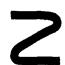
\includegraphics[keepaspectratio]{images/part001_9d1170b3.jpg}}

\begin{enumerate}
\def\labelenumi{\arabic{enumi})}
\setcounter{enumi}{1}
\tightlist
\item
  若 \(f\) 是 \(X\) 到其自身中的连续映射，而 \(g\) 是 \(X\) 到 \(F\) 中的可测映射，则 \(g \circ f\) 未必可测（习题 2）。
\end{enumerate}

推论 1. --- 有限多个可测数值函数（有限或非有限）的上包络与下包络都是可测的。

因为 \(\sup (u,v)\) 与 \(\inf (u,v)\) 在 \(\overline{\mathbf{R}}\times \overline{\mathbf{R}}\) 上连续

推论 2. --- 要使数值函数 \(f\)（有限或非有限）可测，必须且只需 \(f^{+}\) 与 \(f^{-}\) 可测。

条件是必要的，由推论 1 即得；它是充分的，因为 X 在 \(\overline{R} \times \overline{R}\) 中的像 A（在映射 \(x \mapsto (f^{+}(x), f^{-}(x))\) 下）不含点 \((+\infty, +\infty)\) 与 \((-\infty, -\infty)\)，从而映射 \((u, v) \mapsto u - v\) 在 A 上连续。

推论 3. --- 若 f 与 g 是 X 到拓扑向量空间 F 中的两个可测映射，则 \(f + g\) 与 \(\alpha f\) 都是可测的（ \(\alpha\) 为任意标量）。

因此，X 到拓扑向量空间 F 中的可测映射所成之集是一个向量空间。

推论 4. --- 设 F 是 R 上的一个 n 维向量空间，并设 \((\mathbf{e}_{k})_{1\leqslant k\leqslant n}\) 是 F 的一个基。要使函数 \(f=\sum_{k=1}^{n}\mathbf{e}_{k}f_{k}\) 可测，必须且只需每个数值函数 \(f_{k}\) 都可测。

推论 5. --- 设 F、G、H 是三个拓扑向量空间，并设 \((u, v) \to [u \cdot v]\) 是 \(F \times G\) 到 H 中的一个连续双线性映射。若 f 是 X 到 F 中的可测映射，g 是 X 到 G 中的可测映射，则 \([f \cdot g]\) 是 X 到 H 中的可测映射。

特别地，若 f 是 X 到实（相应地，复）赋范空间 F 中的可测映射，而 g 是 X 到 R（相应地，C）中的可测映射，则 gf 可测。若 F 是一个赋范代数，且 f、g 是 X 到 F 中的两个可测映射，则 fg 可测。

推论 6. --- 若 f 是 X 到赋范空间 F 中的可测映射，则数值函数 \(|f|\) 是可测的。

\subsection{可测函数的极限}

定理 2（Egoroff）. --- 设 X 是一个局部紧空间，\(\mu\) 是 X 上的一个测度，A 是一个可数集，F 是 A 上具有可数基的一个滤子，而 \((f_{\alpha})_{\alpha\in\mathbb{A}}\) 是 X 到可度量化空间 F 中的可测映射的一个族。假设 \(\lim_{\mathfrak{F}} f_{\alpha}(x) = f(x)\) 在 X 的一个局部可忽略子集 N 的余集中存在。在这些条件下，

\(1^{\circ}\) 函数 \(f\)（以任意方式延拓到 \(\mathbf{N}\) 上）是可测的；

\(2^{\circ}\) 对 X 的每个紧子集 K 和每个 \(\varepsilon > 0\)，存在紧集 \(\mathrm{K}_{1} \subset \mathrm{K}\)，使得 \(|\mu| (\mathrm{K} - \mathrm{K}_{1}) \leqslant \varepsilon\)，且诸 \(f_{\alpha}\) 到 \(\mathrm{K}_{1}\) 上的限制都连续，且一致收敛于 \(f\)（在 \(\mathrm{K}_{1}\) 上）。

第一个断言显然由第二个断言得出，我们来证明后者。存在紧集 \(K_{0} \subset K\)，使得 \(|\mu|(\mathrm{K} - \mathrm{K}_{0}) \leqslant \varepsilon/2\)，且在 \(K_{0}\) 上所有函数 \(f_{\alpha}\) 的限制都连续（No.~1, 命题 2）。设 \((\mathrm{A}_{n})\) 是滤子 F 的一个递减可数基；设 d 是 F 上与该拓扑相容的一个距离。对每对整数 \(n > 0\)、\(r > 0\)，设 \(\mathbf{B}_{n,r}\) 是点 \(x \in \mathrm{K}_0\)（使得至少有一对指标 \(\alpha, \beta\)（属于 \(\mathbf{A}_n\) 者）满足 \(d(f_{\alpha}(x), f_{\beta}(x)) \geqslant 1 / r\)）所成之集；对固定的 \(\alpha\) 与 \(\beta\)，\(x \in \mathrm{K}_0\)（使得 \(d(f_{\alpha}(x), f_{\beta}(x)) \geqslant 1 / r\) 者）所成之集在 \(\mathbf{K}_0\) 中是闭的，因而是紧的；于是，\(\mathbf{B}_{n,r}\) 是含于 \(\mathbf{K}_0\) 的紧集的一个可数并，从而是可积的（§4, No.~5, 命题 6 与 8）。若固定 \(r\)，则诸集合 \(\mathbf{B}_{n,r}\)（ \(n = 1,2,\ldots\) ）的递减序列的交测度为零，因为 \(f_{\alpha}(x)\) 趋于 \(f(x)\)（在 \(\mathbf{K}_0\) 中关于滤子 \(\mathfrak{F}\) 几乎处处）；于是 \(\lim_{n \to \infty} |\mu|(\mathbf{B}_{n,r}) = 0\)（§4, No.~5, 命题 7 的推论），从而存在整数 \(n_r\)，使得 \(|\mu|(\mathbf{B}_{n_r,r}) \leqslant \varepsilon / 2^{r+2}\)。设 \(B\) 是（对 \(r = 1,2,\ldots\) ）诸集合 \(\mathbf{B}_{n_r,r}\) 的并；\(B\) 是可积的，且

\[
| \mu | (\mathrm{B}) \leqslant \sum_ {r = 1} ^ {\infty} | \mu | (\mathrm{B} _ {n _ {r}, r}) \leqslant \varepsilon / 4
\]

（§4, No.~5, 命题 8 的推论）。设 C 是 B 在 \(K_{0}\) 中的余集；按构造，关于滤子 F，\(f_{\alpha}(x)\) 在 C 中一致收敛于 \(f(x)\)，且由于诸 \(f_{\alpha}\) 到 C 上的限制是连续的，f 到 C 上的限制也是连续的。于是只需取紧集 \(K_{1} \subset C\)，使得 \(|\mu|(\mathrm{C} - \mathrm{K}_{1}) \leqslant \varepsilon/4\)，即可满足陈述的条件，因为 \(|\mu|(\mathrm{K} - \mathrm{K}_{1}) = |\mu|(\mathrm{K} - \mathrm{K}_{0}) + |\mu|(\mathrm{B}) + |\mu|(\mathrm{C} - \mathrm{K}_{1}) \leqslant \varepsilon\)。

若 F 不可度量化，定理 2 的结论未必成立（习题 1）。若 F 可度量化，且集合 A 不可数但滤子 \(\mathfrak{F}\) 具有可数基，则定理 2 的第一个结论仍然有效；因为若 \((\mathrm{A}_n)\) 是 \(\mathfrak{F}\) 的一个可数基，而 \(\alpha_{n}\) 是 \(\mathrm{A}_n\) 的一个元素，则 \(f\) 是序列 \((f_{\alpha_n})\) 局部几乎处处意义下的极限，从而是可测的；然而，定理 2 的第二个结论不再必然成立（参看习题 4）。

推论 1. --- 设 \((f_n)\) 是数值函数（有限或非有限）的一个序列。若诸 \(f_n\) 可测，则函数 \(\sup_{n} f_n\)、\(\inf_{n} f_n\)、\(\limsup_{n \to \infty} f_n\) 与 \(\liminf_{n \to \infty} f_n\) 都是可测的。

因为扩充实直线 \(\overline{\mathbf{R}}\) 同胚于 \(\mathbf{R}\) 的一个紧区间，故它是可度量化的。函数 \(\sup_{n} f_n\) 是递增函数序列 \(g_n = \sup(f_1, f_2, \ldots, f_n)\) 的逐点极限，而这些函数是可测的（No.~3, 定理 1 的推论 1）；类似地，\(\limsup_{n \to \infty} f_n\) 是递减函数序列 \(h_n = \sup_{p \geqslant 0} f_{n+p}\) 的逐点极限，其中每个函数由前所述是可测的。最后，由于 \(\inf_{n} f_n = -\sup_{n} (-f_n)\) 且 \(\liminf_{n \to \infty} f_n = -\limsup_{n \to \infty} (-f_n)\)，这些函数是可测的。

推论 2. --- X 中的可测集构成一个 σ-集环（GT, IX, §6, No.~3）。

因为若 M 与 N 可测，则函数

\[
\varphi_ {\mathrm{M} \cup \mathrm{N}} = \varphi_ {\mathrm{M}} + \varphi_ {\mathrm{N}} - \varphi_ {\mathrm{M}} \varphi_ {\mathrm{N}} \quad \text {and} \quad \varphi_ {\mathrm{M} \cap \mathbf {C N}} = \varphi_ {\mathrm{M}} - \varphi_ {\mathrm{M}} \varphi_ {\mathrm{N}}
\]

依据 No.~3 的定理 1 的推论 3 与推论 5 是可测的。若 \((\mathrm{M}_{n})\) 是可测集的一个序列而 M 是它们的并，则 \(\varphi_{M} = \sup_{n} \varphi_{M_{n}}\) 依据定理 2 的推论 1 是可测的，由此即得该推论。

特别地，由于开集是可测的：

推论 3. --- X 中的 Borel 集（GT, IX, §6, No.~3, 定义 4）对 X 上的每个测度 \(\mu\) 都是 \(\mu\)-可测的。

\subsection{可测性判别法}

当 F 是拓扑向量空间时，每个取值于 F 的、以可测集为底的阶梯函数（§4, No.~9, 定义 4）显然是可测的（No.~3, 定理 1 的推论 3）；这样的函数 f 只取有限多个值，且对每个 \(y \in F\)，\(f(y)\) 是可测的。更一般地，设 F 是任意拓扑空间，f 是 X 到 F 中只取有限多个不同值 \(a_i\)（ \(1 \leqslant i \leqslant m\) ）的一个映射；若诸集合 \(A_i = f(a_i)\) 可测，则函数 f 可测。因为，对每个紧集 K 以及诸集合 \(A_i \cap K\) 中的每一个，存在可忽略集 \(N_i \subset A_i \cap K\) 以及 \(A_i \cap K \cap C N_i\) 的由紧集序列（ \(K_{in}\) ）构成的一个分割；由于 K 是诸集合 \(A_i \cap K\) 的并，且 f 到每个 \(K_{in}\) 上的限制是常数、从而是连续的，故 f 可测。我们约定，按措辞的一种滥用，称 X 到 F 中的映射 f 为可测阶梯函数，如果它只取有限多个值，且对每个 \(y \in F\)，\(f(y)\) 是可测的。

定理 3. --- 要使 X 到可度量化空间 F 中的映射 f 可测，必须且只需：对每个紧集 \(K \subset X\)，存在取值于 F 的可测阶梯函数的一个序列 \((g_{n})\)，使得 \(g_{n}(x)\) 趋于 \(f(x)\)（对几乎所有 \(x \in K\)）。

条件是充分的，由 Egoroff 定理与局部化原理即得。我们来证明它是必要的：由假设，存在可忽略集 \(N \subset K\) 以及由紧集组成的 K - N 的一个分割 \((K_{m})\)，使得 f 到每个 \(K_{m}\) 上的限制是连续的。为定义序列 \((g_{n})\)，只需按如下方式进行：设 d 是与 F 的拓扑相容的一个距离；对每个 \(K_{i}\)（指标满足 \(i \leqslant n\) 者），存在 \(K_{i}\) 分成可积集 \(A_{ij}\)（ \(1 \leqslant j \leqslant q_{i}\) ）的一个有限分割

使得 \(f\) 在每个 \(A_{ij}\) 上的振幅 \(\leqslant 1/n\)（§4, No.~9, 引理）；取 \(g_n\) 在每个 \(A_{ij}\) 上为常数，等于 \(f\) 在该集合中的一个值（对 \(1 \leqslant i \leqslant n\)、\(1 \leqslant j \leqslant q_i\)），等于一个固定元素 \(a \in F\)（对 \(X\) 中不属于任何 \(A_{ij}\) 的每个点）。显然，序列 \((g_n(x))\) 收敛于 \(f(x)\)（在 \(K\) 中每个不属于 \(N\) 的点上）。

推论 1. --- 设 f 是 X 到 Banach 空间 F 中的一个可测映射；对每个紧集 K ⊂ X，存在可测阶梯函数的一个序列 (gₙ)，其支集都含于 K，使得对所有 x ∈ X 有 \textbar gₙ(x)\textbar{} ≤ \textbar f(x)\textbar{}，且对几乎所有 x ∈ K，gₙ(x) 趋于 f(x)。

沿用定理 3 证明中的记号，并用 \(\mathbf{a}_{ij}\) 表示 \(\mathbf{f}\) 在 \(\mathrm{A}_{ij}\) 中的一个值，只需取 \(\mathbf{g}_n\) 在 \(\mathrm{A}_{ij}\) 中的值为：当 \(|\mathbf{a}_{ij}| \leqslant 1/n\) 时取点 0，否则取点 \(\mathbf{a}_{ij}(1 - 1/(n|\mathbf{a}_{ij}|))\)；最后，令 \(\mathbf{g}_n(x) = 0\) 于诸 \(\mathrm{A}_{ij}\)（ \(1 \leqslant i \leqslant n\)，\(1 \leqslant j \leqslant q_i\) ）的并的余集上。

推论 2. --- 设 X 是一个无穷远处可数的局部紧空间。若 f 是 X 到可度量化空间 F 中的可测映射，则存在取值于 F 的可测阶梯函数的一个序列 \((g_{n})\)，使得 \(g_{n}(x)\) 趋于 \(f(x)\)（对几乎所有 \(x \in X\)）。

若 X 是紧集的递增序列 \((\mathbf{A}_{n})\) 的并，则诸非空的集合 \(A_{n}-A_{n-1}\) 构成 X 分成可积集的一个分割；于是，存在可忽略集 \(N\subset X\) 以及由紧集序列 \((\mathrm{K}_{n})\) 构成的 CN 的一个分割，使得 f 到每个 \(K_{n}\) 上的限制是连续的；此后证明可毫无改动地像定理 3 那样完成。

命题 7. --- 设 f 是 X 到拓扑空间 F 中的一个可测映射；F 中每个闭（相应地，开）集在 f 下的逆像是可测的。

只需对 F 中闭集 A 的逆像 \(f(A)\) 进行证明。设 K 是 X 的一个紧子集；存在可忽略集 \(N \subset K\) 以及由紧集组成的 K - N 的一个分割 \((K_n)\)，使得 f 到每个 \(K_n\) 上的限制是连续的。于是交 \(K_n \cap f(A)\) 是闭集 A 在 f 到 \(K_n\) 上的限制下的逆像；因此它是 \(K_n\) 中的闭集，从而是紧的。于是集合 \(K \cap f(A)\) 是可忽略集 \(N \cap f(A)\) 与诸紧集 \(K_n \cap f(A)\) 的并，这就证明了 \(f(A)\) 是可测的。

定理 4. --- 设 F 是一个可度量化空间，d 是 F 上与该拓扑相容的一个距离。要使 X 到 F 中的映射 f 可测，必须且只需它满足下列两个条件：

\begin{enumerate}
\def\labelenumi{\alph{enumi})}
\item
  在 \(f\) 下，\(F\) 的每个闭球的逆像是可测的；
\item
  对每个紧集 \(\mathrm{K} \subset \mathrm{X}\)，存在一个可数子集 \(\mathrm{H}\)（\(\mathrm{F}\) 的），使得 \(f(x) \in \overline{\mathrm{H}}\) 对几乎所有 \(x \in \mathrm{K}\) 成立。
\end{enumerate}

条件 a) 是必要的，由命题 7 即得；另一方面，在定理 3 的记号下，取 H 为由所有函数 \(g_{n}\) 的值组成的可数集，条件 b) 即得到满足。

现在来证明条件 a) 与 b) 是充分的。设 K 是 X 的任意紧子集；存在 K 的一个可忽略子集 N，使得 \(f(\mathrm{K}-\mathrm{N})\) 含于 F 的一个可数点集的闭包中，我们将该点集排成一个序列 \((a_{n})\)。设 \(A_{n,p}\) 是点 \(x \in K-N\)（使得 \(d(f(x), a_{n}) \leqslant 1/p\) 者）所成之集。由条件 a) 可知 \(A_{n,p}\) 是可测的。对固定的 p，递归地定义集合序列 \(B_{n,p} \subset K-N\) 如下：

\[
\mathrm{B} _ {1, p} = \mathrm{A} _ {1, p} \quad \text {and} \quad \mathrm{B} _ {n + 1, p} = \mathrm{A} _ {n + 1, p} \cap \mathbb {C} \Big (\bigcup_ {k \leqslant n} \mathrm{A} _ {k, p} \Big);
\]

诸集合 \(B_{n,p}\) 是可测的，且其中非空者构成 K-N 的一个分割。设 \(g_{m,p}\) 是这样的函数：等于 \(a_{i}\) 于集合 \(B_{i,p}\) 上（对 \(1 \leqslant i \leqslant m\)），在这些集合的并的余集上等于一个常数 \(b \in F\)；\(g_{m,p}\) 是一个可测阶梯函数；当 m 趋于无穷时，\(g_{m,p}\) 逐点收敛于函数 \(f_{p}\)，后者等于 \(a_{n}\) 于 \(B_{n,p}\)（ \(n \geqslant 1\) ）上，在 N∪CK 上等于 b，因此（定理 2）\(f_{p}\) 是可测的。当 p 趋于无穷时，\(f_{p}(x)\) 趋于 \(f(x)\)（对每个 \(x \in K-N\)），而对 \(x \in N \cup CK\) 趋于 b；因此诸 \(f_{p}\) 的极限是可测的，再由局部化原理即知 f 本身是可测的。

注. --- 1) 仅条件 a) 不足以使 \(f\) 可测（习题 7）。

因为，若确实如此，则对每个 \(b \in \overline{R}\)，使 \(f(x) \geqslant b\) 的 x 所成之集是可测的，因为它是使 \(f(x) \geqslant a\) 的 x 所成之集（它们构成一个可数族）的交，其中 a 遍历 D 中 \(\leqslant b\) 的点所成之集。使 \(f(x) < b\) 的 x 所成之集是可测的，因为它是一个可测集的余集。其次，若 b 有限，则使 \(f(x) \leqslant b\) 的 x 所成之集是可测的，因为它是使 \(f(x) < b + 1/n\) 的 x 所成之集的交；而 \(\overline{f}(-\infty)\) 是可测的，因为当 n 遍历 Z 时，它是使 \(f(x) < n\) 的 x 所成之集的交。最后，f 下 \(\overline{R}\) 的每个闭区间的逆像是可测的，因为它是两个可测集的交，于是可以应用定理 4。

同样可以证明，只需对每个 \(a \in D\)，\(x\)（使得 \(f(x) > a\) 者）所成之集是可测的即可。

推论. --- 每个下半（相应地，上半）连续函数都是可测的。

因为若 \(f\) 是下半连续的，则 \(x \in \mathbf{X}\)（使得 \(f(x) \leqslant a\) 者）所成之集对每个 \(a \in \overline{\mathbf{R}}\) 都是闭的。

当 F 可度量化且紧时，命题 7 使我们能将定理 3 加强如下：

命题 9. --- 若 F 是一个可度量化的紧空间，则每个 X 到 F 中的可测映射 f 都是可测阶梯函数序列的（在整个 X 上的）一致极限。

设 \(d\) 是与 \(\mathbf{F}\) 的拓扑相容的一个距离。对每个正整数 \(n\)，存在有限多个点 \(a_{k} \in \mathbf{F}\)，使得闭球 \(\mathbf{B}_{k}\)（以 \(a_{k}\) 为中心、\(1/n\) 为半径）构成 \(\mathbf{F}\) 的一个覆盖；于是诸集合 \(\mathbf{A}_{k} = f(\mathbf{B}_{k})^{-1}\) 是可测的（命题 7）且构成 \(\mathbf{X}\) 的一个覆盖。因此（§4, No.~9, 引理）存在一个分割 \((\mathbf{C}_{i})\)（把 \(\mathbf{X}\) 分成有限多个可测集的），使得每个 \(\mathbf{A}_{k}\) 都是某些 \(\mathbf{C}_{i}\) 的并。设 \(c_{i}\) 是 \(\mathbf{C}_{i}\) 的一个点，并设 \(g_{n}\) 是等于 \(f(c_{i})\) 于 \(\mathbf{C}_{i}\) 上（对每个指标 \(i\)）的可测阶梯函数。显然，\(d(f(x), g_{n}(x)) \leqslant 2/n\) 对所有 \(x \in \mathbf{X}\) 成立。

命题 10. --- 设 F 是一个可分 Banach 空间，F' 是它的对偶，而 (a'\_n) 是 F' 的单位球中的一个弱稠密序列（TVS, III, §3, No.~4, 命题 6 的推论 2）。¹ 要使 X 到 F 中的映射 f 可测，必须且只需对每个 n，标量函数 x ↦ ⟨f(x), a'\_n⟩ 都是可测的。

条件显然是必要的（No.~3, 定理 1），我们来证明它是充分的；只需验证定理 4 的条件 a)，为此，由局部化原理，只需证明：对 X 的每个紧子集 K 以及 F 中每个以 a 为中心、r 为半径的闭球 \(B \subset F\)，集合 \(A = K \cap \mathbf{f}^{-1}(B)\) 都是可测的；而现在，对每个 \(z \in F\)，

\[
| \mathbf {z} | = \sup _ {n} | \langle \mathbf {z}, \mathbf {a} _ {n} ^ {\prime} \rangle | / | \mathbf {a} _ {n} ^ {\prime} |;
\]

于是 A 是 \(K\) 与由下式定义的诸集合的交

\[
\left| \left\langle \mathbf {f} (x), \mathbf {a} _ {n} ^ {\prime} \right\rangle - \left\langle \mathbf {a}, \mathbf {a} _ {n} ^ {\prime} \right\rangle \right| \leqslant r \left| \mathbf {a} _ {n} ^ {\prime} \right|;
\]

由于这些集合依假设是可测的，故 A 是可测的。

推论 1. --- 设 F 是一个 Banach 空间。要使 X 到 F 中的映射 f 可测，必须且只需它满足下列两个条件：

\begin{enumerate}
\def\labelenumi{\alph{enumi})}
\tightlist
\item
  对每个 \(\mathbf{a}' \in \mathrm{F}'\)，标量函数 \(x \mapsto \langle \mathbf{f}(x), \mathbf{a}' \rangle\) 是可测的；
\item
  对每个紧集 \(\mathrm{K} \subset \mathrm{X}\)，存在一个可数子集 \(\mathrm{H}\)（\(\mathrm{F}\) 的），使得 \(\mathbf{f}(x) \in \overline{\mathrm{H}}\) 对几乎所有 \(x \in \mathrm{K}\) 成立。
\end{enumerate}

这些条件的必要性由 No.~3 的定理 1 以及定理 4 得出。为证明条件是充分的，仍只需验证定理 4 的条件 a)。沿用命题 10 证明中的记号，我们可以（借助于 b)）在必要时于一个可忽略集上修改 f 之后，假设 \(\mathbf{f}(\mathrm{K}) \subset \overline{\mathrm{H}}\)，其中 H 是 F 的一个可数子集。若 V 是由集合 \(H \cup \{a\}\) 生成的 F 的闭线性子空间，则 V 是一个可分 Banach 空间，且 V 上每个连续线性形式都是某个形式 \(a' \in F'\) 的限制；于是与命题 10 中同样的推理表明 \(K \cap \overline{\mathbf{f}}(B)\) 是可测的。

推论 2. --- 设 F 是一个可度量化且可分的局部凸空间，并设 \(F'\) 是它的对偶。要使 X 到 F 中的映射 f 可测，必须且只需对每个 \(a' \in F'\)，标量函数 \(x \mapsto \langle \mathbf{f}(x), \mathbf{a}' \rangle\) 都是可测的。

我们可以把 F 视为 Banach 空间的一个可数乘积 \(\prod_{n}E_{n}\) 的子空间（TVS, II, §4, No.~3），并且可以假设 \(\operatorname{pr}_{n}(\mathbf{F})\) 在 \(E_{n}\) 中稠密，后者因而是可分的。这样，对每个 n，映射 \(pr_{n}\circ f\) 依据命题 10 是可测的，因此 f 依据 No.~3 的定理 1 是可测的。

命题 11. --- 设 F 是一个局部凸空间，它是可分且可度量的局部凸空间的一个序列 \(F_{n}\) 的直接极限，且 F 是诸 \(F_{n}\) 的并。设 \(F'\) 是 F 的对偶，赋以弱拓扑 \(\sigma(\mathrm{F}',\mathrm{F})\)。要使 X 到 \(F'\) 中的映射 f 可测，必须且只需：对每个 \(a \in F\)，标量函数 \(x \mapsto \langle \mathbf{a}, \mathbf{f}(x) \rangle\) 都是可测的。

条件是必要的，由 No.~3 的定理 1 即得；我们来证明它是充分的。首先假设 F 可度量化且可分，并设 D 是 F 中的一个可数稠密集。设 \((\mathrm{V}_{n})\) 是 F 中 0 的均衡凸开邻域的一个递减基本序列；极集 \(V_{n}^{\circ}\) 是等度连续的，且它们的并就是整个 \(F'\)。设 \(X_{n} = \overline{\mathbf{f}}(V_{n}^{\circ})\)；序列 \((\mathrm{X}_{n})\) 是递增的，且 \(X = \bigcup_{n} X_{n}\)；我们来证明每个 \(X_{n}\) 都是 \(\mu\)-可测的。事实上，\(D \cap V_{n}\) 在 \(V_{n}\) 中稠密；对每个 \(y \in D \cap V_{n}\)，设 \(S_{y}\) 是 \(x \in X\)（使得 \(|\langle y, f(x) \rangle| \leqslant 1\) 者）所成之集；假设蕴含每个 \(S_{y}\) 都可测，而 \(X_{n}\) 是诸 \(S_{y}\)（对 \(y \in D \cap V_{n}\)）组成的可数族的交。在此基础上，对 X 的每个紧子集 K 和每个 \(\varepsilon > 0\)，存在整数 n，使得 \(|\mu| (K - (K \cap X_{n})) \leqslant \varepsilon/4\)，然后存在紧子集 \(K_{1}\)（\(K \cap X_{n}\) 的），使得 \(|\mu| ((K \cap X_{n}) - K_{1}) \leqslant \varepsilon/4\)；最后，存在紧子集 \(K_{2}\)（\(K_{1}\) 的），使得 \(|\mu| (K_{1} - K_{2}) \leqslant \varepsilon/2\)，且在 \(K_{2}\) 上所有函数 \(\langle y, f \rangle\)（其中 \(y \in D\)）的限制都是连续的（No.~1, 命题 2）。由于集合 \(f(K_{2}) \subset f(X_{n}) \subset V_{n}^{\circ}\) 是等度连续的，\(\sigma(F', F)\) 在 \(f(K_{2})\) 上诱导的拓扑与在 D 上逐点收敛的拓扑相同（GT, X, §2, No.~4, 定理 1）；因此 f 到 \(K_{2}\) 上的限制是连续的，由此得到第一种情形下的断言。

现在过渡到一般情形。若 \(\mathbf{z}'\) 是 \(\mathbf{F}\) 上的一个连续线性形式，则其限制 \(\mathbf{z}_n'\)（到 \(\mathbf{F}_n\) 上的）是连续的；由于 \(\mathbf{F} = \bigcup_{n} \mathbf{F}_n\)，对偶 \(\mathbf{F}'\)（\(\mathbf{F}\) 的）可以（在代数意义上）等同于乘积 \(\prod_{n} \mathbf{F}_n'\) 的一个线性子空间，且此时 \(\operatorname{pr}_n(\mathbf{z}') = \mathbf{z}_n'\)。此外，由于 \(\mathbf{F}\) 的每个有限子集都含于某个 \(\mathbf{F}_n\)，拓扑 \(\sigma(\mathbf{F}', \mathbf{F})\) 恰是诸拓扑 \(\sigma(\mathbf{F}_n', \mathbf{F}_n)\) 的乘积拓扑所诱导的拓扑。在此基础上，若 \(\langle \mathbf{a}, \mathbf{f} \rangle\) 对每个 \(\mathbf{a} \in \mathbf{F}\) 可测，则 \(\langle \mathbf{a}_n, \operatorname{pr}_n \circ \mathbf{f} \rangle\) 对每个 \(n\) 与每个 \(\mathbf{a}_n \in \mathbf{F}_n\) 也可测，因为 \(\langle \mathbf{a}_n, \operatorname{pr}_n \circ \mathbf{f} \rangle = \langle \mathbf{a}_n, \mathbf{f} \rangle\)；于是证明的第一部分表明，\(\operatorname{pr}_n \circ \mathbf{f}\) 对每个 \(n\) 可测，因此 \(\mathbf{f}\) 也可测（No.~3, 定理 1）。

\subsection{可积性判别法}

定理 5. --- 要使 X 到 Banach 空间 F 中的映射 f 是 p 次幂可积的（ \(1 \leqslant p < +\infty\) ），必须且只需 f 可测且 \(N_{p}(\mathbf{f})\) 有限。

条件是必要的：因为若 \(f \in L_{F}^{p}\)，则存在具有紧支集的连续函数的一个序列 \((\mathbf{g}_{n})\)，它几乎处处收敛于 f（§3, No.~4, 定理 3 的推论 2）；由 No.~4 的定理 2，f 是可测的。

为证明条件是充分的，我们先建立一条引理：

引理 1. --- 设 g 是取值于 F 的一个函数，使得 \(\mathrm{N}_{p}(\mathbf{g}) < +\infty\)（换言之，\(F_{F}^{p}\) 中的一个函数）。点 \(x \in X\)（使得 \(\mathbf{g}(x) \neq 0\) 者）所成之集 A 含于一个可忽略集与一个紧集序列的并。

设 \(A_{n}\) 是点 \(x \in X\)（使得 \(|\mathbf{g}(x)| \geqslant 1/n\) 者）所成之集；A 是诸 \(A_{n}\) 的并，且 \(\varphi_{A_{n}} \leqslant n|\mathbf{g}|\)，于是 \(|\mu|^{*}(A_{n}) \leqslant (nN_{p}(\mathbf{g}))^{p}\)；由此可知 \(A_{n}\) 含于一个可忽略集与一个紧集序列的并（§4, No.~6, 定理 4 的推论 3），因此 A 亦然。

引理证毕后，先考虑 \(\mathbf{f}\) 具有紧支集 \(\mathbf{K}\) 的情形。由 No.~5 的定理 3 的推论 1，存在可测阶梯函数的一个序列 \((\mathbf{g}_n)\)，使得 \(|\mathbf{g}_n(x)| \leqslant |\mathbf{f}(x)|\)（在每一点 \(x \in \mathbf{X}\) 处），且 \(\mathbf{g}_n(x)\) 几乎处处趋于 \(\mathbf{f}(x)\)。而现在，\(\mathbf{g}_n\) 是含于 \(\mathbf{K}\) 的可测集的特征函数的一个线性组合；由于这些集合依据 No.~1 的命题 3 是可积的，故 \(\mathbf{g}_n\) 属于 \(\mathcal{L}_{\mathrm{F}}^p\)。由于 \(\mathrm{N}_p(\mathbf{f}) < +\infty\)，Lebesgue 定理（§3, No.~7, 定理 6）表明 \(\mathbf{f}\) 属于 \(\mathcal{L}_{\mathrm{F}}^p\)。

在一般情形下，由引理 1 可知存在紧集的一个递增序列 \((\mathrm{K}_n)\)，使得 \(\mathbf{f}(x)\) 在诸 \(\mathrm{K}_n\) 的并的余集中几乎处处为零。设 \(\mathbf{f}_n\) 是等于 \(\mathbf{f}(x)\) 于 \(\mathrm{K}_n\) 上、在其他处等于 0 的函数；\(\mathbf{f}_n\) 依据 No.~3 的定理 1 的推论 5 是可测的；由于 \(|\mathbf{f}_n| \leqslant |\mathbf{f}|\)，由论证的第一部分知 \(\mathbf{f}_n\) 属于 \(\mathcal{L}_{\mathrm{F}}^p\)。由于 \(\mathbf{f}(x)\) 几乎处处等于序列 \(\mathbf{f}_n(x)\) 的极限，Lebesgue 定理再次证明 \(\mathbf{f} \in \mathcal{L}_{\mathrm{F}}^p\)，证明至此完成。

应当注意，一个局部可忽略但并非可忽略的函数不是可积的；因此，与一个可积函数局部几乎处处相等的函数未必可积。

推论 1. --- 要使一个集合可积，必须且只需它是可测的且外测度有限。

推论 2. --- 设 \((\mathrm{F}_{n})\) 是拓扑空间的一个序列；对每个指标 n，设 \(f_{n}\) 是 X 到 \(F_{n}\) 中的可测映射，并设 \(f(x) = (f_{n}(x)) \in \mathrm{F} = \prod_{n} \mathrm{F}_{n}\)；最后，设 u 是 \(f(\mathrm{X})\) 到 Banach 空间 G 中的一个连续映射。要使函数 \(\mathbf{g}(x) = \mathbf{u}(f(x))\) 可积，必须且只需 \(\mathrm{N}_{1}(\mathbf{g}) < +\infty\)。

因为 \(\mathbf{g}\) 是可测的（No.~3, 定理 1）。

推论 3. --- 对每个可积函数 f 与每个可测集 A，函数 \(f\varphi_{A}\) 是可积的。

因为由定理 5 与 No.~3 的定理 1 的推论 5 可知 \(\mathbf{f}\varphi_{\mathrm{A}}\) 是可测的，且 \(\mathrm{N}_1(\mathbf{f}\varphi_{\mathrm{A}}) \leqslant \mathrm{N}_1(\mathbf{f})\)。

我们记 \(\int_{\mathrm{A}} \mathbf{f} d\mu = \int \mathbf{f} \varphi_{\mathrm{A}} d\mu\)（或 \(\int_{\mathrm{A}} \mathbf{f} \mu\)），对每个可积函数 \(\mathbf{f}\) 与每个可测集 \(\mathrm{A}\)。我们也用 \(\int_{\mathrm{A}}^{*} f d|\mu|\)（或 \(\int_{\mathrm{A}}^{*} f |\mu|\)）来代替 \(\int^{*} f \varphi_{\mathrm{A}} d|\mu|\)，对每个数值函数（有限或非有限的）\(f \geqslant 0\)（约定 \(f(x) \varphi_{\mathrm{A}}(x) = 0\) 当 \(f(x) = +\infty\) 且 \(\varphi_{\mathrm{A}}(x) = 0\) 时）。

推论 4. --- 对每个序列 \((f_{n})\)（由 X 上 \(\geqslant 0\) 的可测函数组成），

\[
\int^ {*} \left(\sum_ {n} f _ {n}\right) d | \mu | = \sum_ {n} \int^ {*} f _ {n} d | \mu |.\tag{1}
\]

鉴于 §1, No.~3, 定理 3，我们归结为证明：对任意两个可测函数 \(f \geqslant 0\)、\(g \geqslant 0\)（\(X\) 上的），

\[
\int^ {*} (f + g) d | \mu | = \int^ {*} f d | \mu | + \int^ {*} g d | \mu |.\tag{2}
\]

当 \(f\) 与 \(g\) 可积时，这只是积分的可加性。在相反的情形，例如若 \(f\) 不可积，则由定理 5 有 \(\int^{*} f d|\mu| = +\infty\)；更有 \(\int^{*}(f + g) d|\mu| = +\infty\)。

推论 5. --- 对两两不相交的可测集的每个序列 \((\mathbf{A}_{n})\)，

\[
| \mu | ^ {*} \left(\bigcup_ {n} \mathrm{A} _ {n}\right) = \sum_ {n} | \mu | ^ {*} (\mathrm{A} _ {n}).
\]

这由推论 4 应用于诸 \(\varphi_{\mathrm{A}_n}\) 即得。
